\chapter{Champ additif\\et multiplicatif} \label{Num3}

\begin{prerequis}[Dans les programmes - cycle 1]
   {\bf Découvrir les nombres et leurs utilisations}
   \begin{itemize}
     \item Avoir compris que tout nombre s'obtient en ajoutant un au nombre précédent et que cela correspond à l'ajout d'une unité à la quantité précédente.
      \item Quantifier des collections jusqu'à dix au moins ; les composer et les décomposer par manipulations effectives puis mentales.
      \item Dire combien il faut ajouter ou enlever pour obtenir des quantités ne dépassant pas dix.
      \item Parler des nombres à l'aide de leur décomposition.
   \end{itemize}
\end{prerequis}

\begin{prerequis}[Dans les programmes - cycle 2]
{\bf Calculer avec des nombres entiers}
   \begin{itemize}
      \item Calcul posé : mise en \oe uvre d'un algorithme de calcul posé pour l'addition, la soustraction, la multiplication.
   \end{itemize}
\end{prerequis}
  
\begin{prerequis}[Dans les programmes - cycle 3]
{\small
{\bf Calculer avec des nombres entiers et des nombres décimaux}
   \begin{itemize}
      \item Connaître et mettre en œuvre un algorithme de calcul posé pour effectuer : \\
         -- l’addition, la soustraction et la multiplication de nombres entiers ou décimaux ; \\
         -- la division euclidienne d’un entier par un entier ; \\
         -- la division d’un nombre décimal (entier ou non) par un nombre entier. 
      \item Calcul instrumenté : Utiliser une calculatrice pour trouver ou vérifier un résultat.
\end{itemize}
   }
\end{prerequis}

\vfill

%%%%%%%%%%%%%%%%%%%%%%%%%%
%%%%%%%%%%%%%%%%%%%%%%%%%%
\reperes

%%%%%%%%%%%%%
\section{Le champ additif}
%%%%%%%%%%%%%

Le champ additif réunit à lui seul les additions et les soustractions. Mais le choix et l'application de l'une ou l'autre de ces opérations n'est pas forcément simple pour les élèves.


\subsection{Classification des problèmes à structure additive} %%%

Selon {\it Gérard Vergnaud} [ver86], on peut classer les problèmes à structures additives selon six types dont les quatre suivants sont les plus utilisés :

{\bf La composition de deux états : $\syst{\square}{\square}\square$}

   \begin{tabular}{|m{4.5cm}|m{9cm}|m{1.8cm}|}
      \hline
      Recherche du composé &
      Noé a 7 billes rouges et 4 billes bleues, combien a-t-il de billes au total ? &
      $\syst{7}{4}\,\square$ \\
      \hline
      Recherche d'une partie & Noé a 11 billes de couleurs bleues et rouges. Il possède 7 billes rouges, combien a-t-il de billes bleues ? & $\syst{7}{\square}$\,11 \\
      \hline
   \end{tabular}
      
\medskip
      
{\bf La transformation d'un état} : $\rnode{a}{\square}\,\to\,\rnode{b}{\square} \ncangles[angleA=90,angleB=90,linearc=.2,arrows=->]{a}{b} \ncput*{\bigcirc}$ \\ [-3mm]
   
   \begin{tabular}{|m{4.5cm}|m{9cm}|m{1.8cm}|}
      \hline
      Recherche de l'état final &
      Noé avait 25 billes, il en a gagné 7 pendant la récréation. Combien en a-t-il maintenant ? &
      \begin{pspicture}(0,0)(1.5,1) 
         \psset{nodesep=4pt}
         $\rnode{a}{25\phantom{\square}}\hspace*{0.3cm}\to\hspace*{0.3cm}\rnode{b}{\square}
          \ncangles[angleA=90,angleB=90,linearc=.4,arrows=->]{a}{b}
         \ncput*{+7}$
      \end{pspicture} \\
      \hline
      Recherche de l'état initial &
      Noé a gagné 7 billes pendant la récréation. Il en a maintenant 32. Combien en avait-il avant ? &
      \begin{pspicture}(0,0)(1.5,1)
         \psset{nodesep=4pt}
         $\rnode{a}{\square\phantom{\square}}\hspace*{0.3cm} \to\hspace*{0.3cm} \rnode{b}{32}
         \ncangles[angleA=90,angleB=90,linearc=0.4,arrows=->]{a}{b}
         \ncput*{+7}$
      \end{pspicture} \\
      \hline
      Recherche de la transformation &
      Noé avait 25 billes avant la récréation, il en a maintenant 32. Combien en a-t-il gagné ? &
      \begin{pspicture}(0,0)(1.5,1)
         \psset{nodesep=4pt}
         $\rnode{a}{25}\hspace*{0.3cm} \to\hspace*{0.3cm} \rnode{b}{\scriptstyle{32}}
         \ncangles[angleA=90,angleB=90,linearc=0.4,arrows=->]{a}{b}
         \ncput*{\bigcirc}$
      \end{pspicture} \\
      \hline
   \end{tabular}
   
\smallskip
    
{\bf La comparaison des états} : \begin{minipage}{1cm} $\rnode{a}{\square} \\ \ \\ \rnode{b}{\square} \ncline{a}{b} 
\naput{\bigcirc}$ \end{minipage}
   
   \begin{tabular}{|m{4.5cm}|m{9cm}|m{1.8cm}|}
      \hline
      Recherche de l'un des états &
      Noé a 32 billes, il en a 7 de plus que Matéo. Combien de billes a Matéo ? &
      \begin{minipage}{1cm}
         $\rnode{a}{32} \\
         \ \\
         \rnode{b}{\;\square\;}
         \ncline{a}{b} \naput{-7}$
      \end{minipage} \\ [5mm]
      \hline
      Recherche de la comparaison &
      Noé a 32 billes, Matéo en a 25. Combien de billes Matéo a-t-il en moins que Noé ? &
      \begin{minipage}{1cm}
         $\rnode{a}{32} \\
         \ \\
         \rnode{b}{25}
         \ncline{a}{b} \naput{\bigcirc}$
      \end{minipage} \\ [5mm]
      \hline
   \end{tabular}
 
   
{\bf La composition de transformations} : \begin{pspicture}(0,-0.3)(2,0.7) \pscircle(0.5,0.3){0.15} \pscircle(1.5,0.3){0.15} \psline{->}(0.2,0)(0.8,0) \psline{->}(1.2,0)(1.8,0) \psline{->}(0.2,-0.3)(1.8,-0.3) \pscircle(1,-0.6){0.15} \end{pspicture} \\
   
  \begin{tabular}{|p{4.5cm}|p{9cm}|p{1.8cm}|}
      \hline
      Recherche de la transformation composée &
      Noé a joué deux parties de billes. Il en a gagné 8 à la première partie et en a perdu 3 à la seconde. Combien a-t-il gagné de billes au total ? &
     \begin{pspicture}(0.2,0.1)(2,0.7) 
         \rput(0.5,0.3){$+8$}
         \rput(1.5,0.3){$-3$}
         \psline{->}(0.2,0)(0.8,0)
         \psline{->}(1.2,0)(1.8,0)
         \psline{->}(0.2,-0.3)(1.8,-0.3)
         \pscircle(1,-0.6){0.15}
         \end{pspicture} \\ [5mm]
      \hline
      Recherche de l'une des composantes &
      Noé a joué deux parties de billes. Il en a gagné 8 à la première partie et en a gagné 5 au total. Combien en a-t-il perdu à la seconde partie ? &
      \begin{pspicture}(0.2,0.1)(2,0.7)
         \rput(0.5,0.3){$+8$}
         \pscircle(1.5,0.3){0.15}
         \psline{->}(0.2,0)(0.8,0)
         \psline{->}(1.2,0)(1.8,0)
         \psline{->}(0.2,-0.3)(1.8,-0.3)
         \rput(1,-0.6){$+5$}
      \end{pspicture} \\ [5mm]
      \hline
   \end{tabular}

\pagebreak


\subsection{Le calcul posé en colonnes : l'addition}%%%

Les opérations posées permettent l’obtention de résultats notamment lorsque le calcul mental ou écrit en ligne atteint ses limites. Leur apprentissage est aussi un moyen de renforcer la compréhension du système décimal de position et de consolider la mémorisation des relations numériques élémentaires. Il a donc lieu lorsque les élèves se sont approprié des stratégies de calcul basées sur des décompositions/recompositions. \medskip

{\bf Progressivité des apprentissages}
\begin{description}
   \item[Au CP :] au plus tard en P4, les élèves apprennent à poser les additions en colonnes (nombres à deux chiffres).
   \item[Au CE1 :] ils consolident la maîtrise de l’addition avec des nombres plus grands et de taille différente.
   \item[Au CM1 :] ils étendent aux nombres décimaux l'algorithme de l'addition.
\end{description}

On peut introduire la présentation des calculs en colonne comme une réorganisation du calcul en ligne. Cette nouvelle présentation des calculs est plus économique sur le plan des écritures mathématiques, mais elle est plus délicate à faire fonctionner lorsque le calcul comporte des retenues. Les élèves apprennent à dérouler l'algorithme, c'est-à-dire la suite des calculs de manière automatique.
   
\begin{exemple*1}
   Calcul de $65+17$ : \; \opadd[voperation=top]{65}{17} \; $\to$ le calcul de $5+7$ donne 12, soit 1 dizaine et 2 unités.
\end{exemple*1} \smallskip
   
   Des outils tels que le matériel multibase ou les abaques à jetons, utilisés en fil rouge, peuvent aider à la conceptualisation et à la compréhension de la numération et de l'algorithme de l'addition.
   
\begin{exemple*1}
   Effectuer la somme de 65 et de 17 à l'abaque romain : \\
   {\psset{unit=0.25}
   \begin{pspicture}(3.5,9)(17,24.5)
      \multido{\i=4+4}{4}{\psline(\i,12)(\i,24)}
      \psline(4,24)(16,24)
      \psline(4,22)(16,22)
      \rput(14,23){I}
      \rput(10,23){X}
      \rput(6,23){C}
      \psdots[linecolor=A1](10,21)(11,21)(11,20)(10.5,19)(9.5,19)(10,18)
      \psdots[linecolor=A1](15,21)(14.5,20)(13.5,20)(14,19)(15,19)
      \psdot[linecolor=B1](10,15)
      \psdots[linecolor=B1](14,16)(15,15)(15,15)(14.5,14)(13.5,14)(14,13)(15,13)(15.5,16.5)
      \rput(10,10){\parbox{3.5cm}{\small représentation des\\deux nombres 65 et 17}}
   \end{pspicture}
   \begin{pspicture}(3.5,9)(17,25)
      \multido{\i=4+4}{4}{\psline(\i,12)(\i,24)}
      \psline(4,24)(16,24)
      \psline(4,22)(16,22)
      \rput(14,23){I}
      \rput(10,23){X}
      \rput(6,23){C}
      \psdots(10,21)(11,21)(11,20)(10.5,19)(9.5,19)(10,18)
      \psdots(15,21)(14.5,20)(13.5,20)(14,19)(15,19)
      \psdot(10,17)
      \psdots(14,18)(15,18)(15,18)(14.5,17)(13.5,17)(14,16)(15,16)(14.5,14.7)
      \rput(10,10){\parbox{2.5cm}{\small \og ajout \fg{} des\\deux nombres}}
   \end{pspicture}
   \begin{pspicture}(3.5,9)(17,25)
      \multido{\i=4+4}{4}{\psline(\i,12)(\i,24)}
      \psline(4,24)(16,24)
      \psline(4,22)(16,22)
      \rput(14,23){I}
      \rput(10,23){X}
      \rput(6,23){C}
      \psdots(10,21)(11,21)(11,20)(10.5,19)(9.5,19)(10,18)
      \psdots(15,21)(14.5,20)(13.5,20)(14,19)(15,19)
      \psdot(10,17)
      \psdots(14,18)(15,18)(15,18)(14.5,17)(13.5,17)(14,16)(15,16)(14.5,14.7)
      \psellipse[linecolor=J1](14.2,18)(1.6,2.8)
      \psline[linecolor=J1]{->}(12.6,18)(11,17.5)
      \rput(10,10){\parbox{3cm}{\small échange de 10 unités contre 1 dizaine}}
   \end{pspicture}
   \begin{pspicture}(3.5,9)(15,25)
      \multido{\i=4+4}{4}{\psline(\i,12)(\i,24)}
      \psline(4,24)(16,24)
      \psline(4,22)(16,22)
      \rput(14,23){I}
      \rput(10,23){X}
      \rput(6,23){C}
      \psdots(10,21)(11,21)(11,20)(10.5,19)(9.5,19)(10,18)
      \psdot(10,17)
      \psdots(13.5,18)(14.5,19)
      \psdot[linecolor=J1](11,17.5)
      \rput(10,10){\parbox{2cm}{\small lecture de la somme : 82}}
   \end{pspicture}}
\end{exemple*1}

\smallskip

{\renewcommand{\StringDOCUMENTATION}{Difficultés rencontrées par les élèves :}
\begin{documentation}
   \begin{itemize}
      \item {\bf Connaissance des tables d'addition} : de nombreuses erreurs observées chez les élèves sont liées à une maîtrise insuffisante de ces répertoires.
      \item {\bf Nombres en jeux} : selon la taille et la nature des nombres, les élèves peuvent ne pas maitriser le système de numération, et ne pas comprendre le fonctionnement de l'algorithme.
      \item {\bf Chronologie des calculs} : lorsque les deux termes de l'opération ont le même nombre de chiffres, les élèves mettent en \oe uvre une chronologie qui consiste à calculer de gauche à droite, comme on lit. Ce n'est pas faux, mais cela pose des problèmes avec les retenues.
      \item {\bf Alignement erroné des chiffres} : lorsque les nombres utilisés n'ont pas la même longueur, il peuvent avoir des difficultés à aligner correctement les chiffres.
      \item {\bf Gestion des retenues} : retenue oubliée, inversion du chiffre des dizaines et des unités, retenue écrite mais non prise en compte, retenues systématiques, retenue qui dépasse 1. \\ [-8mm]
   \end{itemize}
\end{documentation}}

\pagebreak


\subsection{Le calcul posé en colonnes : la soustraction}%%%

{\bf Progressivité des apprentissages}
\begin{description}
   \item[Au CE1 :] les élèves apprennent une technique de calcul posé pour la soustraction au plus tard en P3. Le choix de la technique est laissé, en général, aux équipes d’écoles.
   \item[Au CE2 :] ils consolident la maîtrise de la technique de la soustraction apprise en CE1.
   \item[Au CM1 :] ils étendent aux nombres décimaux la technique de la soustraction.
\end{description}

\smallskip


Outre l'addition à trous, il existe actuellement deux techniques utilisées dans les écoles : la technique \og par compensation \fg{} et la technique \og par emprunts \fg{}, encore appelée \og par cassage \fg \\
Dans la technique {\bf par compensations}, les élèves vont apprendre à retirer, rang après rang, le chiffre d'en bas au chiffre d'en haut. Lorsqu'à un rang donné le chiffre d'en haut est inférieur à celui d'en bas, on ajoute dix unités du rang considéré au chiffre d'en haut et une unité au chiffre du rang suivant en bas. Cette technique repose sur la propriété des différences égales puisqu'on ajoute le même nombre 10 aux deux termes de la différence, ce qui ne modifie pas le résultat. Mathématiquement, cela s'écrit $a-b =(a+10)-(b+10)$. La compréhension de la technique classique est souvent problématique car la propriété des différences égales reste assez abstraite. \\   
Pour la technique {\bf par emprunts}, le calcul est posé en colonnes de la même manière. En revanche, lorsqu'à un rang donné le chiffre d'en haut est inférieur à celui d'en bas, on \og emprunte \fg{} une unité du rang supérieur du nombre du haut, qui se transforme en 10 unités de l'ordre considéré. \\
Cette technique utilise le principe des échanges pour traiter les retenues. Elle est considérée comme plus simple à comprendre et à assimiler pour les élèves. En revanche, son écriture devient un peu compliquée lorsque le nombre le plus grand comporte un ou plusieurs 0. C'est aussi la méthode qui n'a souvent pas été apprise par les parents\dots{}
   
\begin{exemple}[0.25]
   Calculer $65-17$.
   \correction
      \vspace*{-5mm}
      \hspace*{2cm}
      $-$\begin{tabular}{lll}
         \multicolumn{3}{l}{\small compensations} \\ [-1mm]
         \phantom{\scriptsize{5}} & & \\ [-1mm]
         6 & {\scriptsize\textcolor{B1}{1}}5 & \\
         1 & 7 \\ [-2mm]
         {\scriptsize\textcolor{B1}{+1}} & & \\
         \cline{1-2}
         4 & 8 & \\
      \end{tabular} 
      \hspace*{2cm}
      $-$\begin{tabular}{cr}
         \multicolumn{2}{c}{\small emprunts} \\ [-1mm]
         \scriptsize{\textcolor{B1}{5}} & \\ [-1mm]
         \cancel{6} & {\scriptsize\textcolor{B1}{1}}5 \\
         1 & 7 \\ [-2mm]
         \phantom{\scriptsize\textcolor{B1}{+1}} & \\
         \hline
         4 & 8 \\
      \end{tabular}
\end{exemple}

\medskip

Là aussi, l'utilisation d'un abaque peut permettre de modéliser la soustraction.

\begin{exemple*1}
   Calcul de $65-17$ à l'abaque romain selon la méthode par emprunts : \\
   {\psset{unit=0.25}
   \begin{pspicture}(3.5,6)(17,24.5)
      \multido{\i=4+4}{4}{\psline(\i,11)(\i,24)}
      \psline(4,24)(16,24)
      \psline(4,22)(16,22)
      \rput(14,23){I}
      \rput(10,23){X}
      \rput(6,23){C}
      \psdots[linecolor=A1](10,21)(11,21)(11,20)(10.5,19)(9.5,19)(10,18)
      \psdots[linecolor=A1](15,21)(14.5,20)(13.5,20)(14,19)(15,19)
      \psdot[linecolor=B1](10,15)
      \psdots[linecolor=B1](14,16)(15,15)(14.5,14)(13.5,14)(14,13)(15,13)(15.5,16.5)
      \rput(10,8){\parbox{3cm}{\small représentation\\des deux nombres\\65 et 17}}
   \end{pspicture}
   \begin{pspicture}(3.5,6)(17,24.5)
      \multido{\i=4+4}{4}{\psline(\i,11)(\i,24)}
      \psline(4,24)(16,24)
      \psline(4,22)(16,22)
      \rput(14,23){I}
      \rput(10,23){X}
      \rput(6,23){C}
      \psdots[linecolor=A1](10,21)(11,21)(11,20)(10.5,19)(9.5,19)(10,18)
      \pscircle[linecolor=J1](11,21){0.5}
      \psline[linecolor=J1]{->}(11,21)(12.5,20.5)
      \psdots[linecolor=J1](13,21)(14,21)(15,21)(13.5,20.5)(14.5,20.5)(15.5,20.5)(13,20)(14,20)(15,20)(13.5,19.5)
      \psdots[linecolor=A1](15,19)(14.5,18)(13.5,18)(14,17)(15,17)
      \psdot[linecolor=B1](10,15)
      \psdots[linecolor=B1](14,15)(15,14)(14.5,13)(13.5,13)(14,12)(15,12)(15.5,15.5)
      \rput(10,8){\parbox{3.1cm}{\small emprunt d'1 dizaine,\\transformation\\en 10 unités}}
   \end{pspicture}
   \begin{pspicture}(3.5,6)(17,24.5)
      \multido{\i=4+4}{4}{\psline(\i,11)(\i,24)}
      \psline(4,24)(16,24)
      \psline(4,22)(16,22)
      \rput(14,23){I}
      \rput(10,23){X}
      \rput(6,23){C}
      \psdots[linecolor=A1](10,21)(11,20)(10.5,19)(9.5,19)(10,18)
      \psdots[linecolor=A1](13,21)(14,21)(15,21)(13.5,20.5)(14.5,20.5)(15.5,20.5)(13,20)(14,20)(15,20)(13.5,19.5)
      \psdots[linecolor=A1](15,19)(14.5,18)(13.5,18)(14,17)(15,17)
      \psdot[linecolor=B1](10,15)
      \psdots[linecolor=B1](14,15)(15,14)(14.5,13)(13.5,13)(14,12)(15,12)(15.5,15.5)
      \rput(10,18){/}
      \rput(10,15){/}
      \psdots[dotstyle=+,linewidth=0.6mm](14,15)(15,14)(14.5,13)(13.5,13)(14,12)(15,12)(15.5,15.5)
      \psdots[dotstyle=+,linewidth=0.6mm](15,19)(14.5,18)(13.5,18)(14,17)(15,17)(15,20)(13.5,19.5)
      \rput(12,9){\parbox{3cm}{\small soustraction\\terme à terme}}
   \end{pspicture}
   \begin{pspicture}(3.5,6)(14,24.5)
      \multido{\i=4+4}{4}{\psline(\i,11)(\i,24)}
      \psline(4,24)(16,24)
      \psline(4,22)(16,22)
      \rput(14,23){I}
      \rput(10,23){X}
      \rput(6,23){C}
      \psdots(10,21)(11,20)(10.5,19)(9.5,19)
      \psdots(13,21)(14,21)(15,21)(13.5,20.5)(14.5,20.5)(15.5,20.5)(13,20)(14,20)
      \rput(12,9){\parbox{3cm}{\small lecture de la\\différence : 48}}
   \end{pspicture}}
\end{exemple*1}

\medskip

{\renewcommand{\StringDOCUMENTATION}{Difficultés rencontrées par les élèves :}
\begin{documentation}
   Les difficultés sont les mêmes que pour les additions, auxquelles on peut ajouter le {\bf choix et la compréhension de la technique} : en CE1, la classe apprend un technique, ensuite, des élèves ayant appris des méthodes différentes peuvent se retrouver dans la même classe.
\end{documentation}}


%%%%%%%%%%%%%%%
\section{Le champ multiplicatif}
%%%%%%%%%%%%%%%

   Le champ des structures multiplicatives concerne les problèmes qui peuvent être résolus en utilisant une multiplication, une division ou une suite de multiplications et de divisions.

\subsection{Classification des structures multiplicatives} %%%

   Il existe plusieurs manières de classer les problèmes qui peuvent se résoudre par une multiplication ou une division. Les tableaux suivants fournissent une classification possible, inspirée de {\it Gérard Vergnaud} [ver86] : il distingue les situations multiplicatives en fonction des grandeurs en jeu et du type de relation qui les relient.
   
   
{\bf Situations portant sur un seul domaine de grandeur} \\ [1mm]
{\hautab{1.2}{
\begin{Ltableau}{\linewidth}{3}{m{5cm}|m{8.5cm}|C{2}}
   \hline
   Problème avec rapport scalaire
   &
   &
   $\square \, \overset{\bigcirc}{\to} \, \square$ \\
   \hline
   Recherche de l'état final 
   &
   Quentin a 7 ans. Son père est quatre fois plus âgé que lui. Quel est l'âge du père ?
   &
   $7 \, \overset{\times4}{\to} \, ?$ \\
   \hdashline
   Recherche de l'état initial  
   &
   Le père de Quentin est quatre fois plus âgé que lui : il a 28 ans. Quel est l'âge de Quentin ?
   &
   $? \, \overset{\times4}{\to} \, 28$ \\
   \hdashline
   Recherche de la transformation
   &
   Quentin a 7 ans. Son père a 28 ans. Combien de fois le père de Quentin est-il plus âgé que lui ?
   &
   $7 \, \overset{?}{\to} \, 28$ \\
   \hline
\end{Ltableau}}}

{\hautab{1.2}{
\begin{Ltableau}{\linewidth}{3}{m{5cm}|m{8.5cm}|m{2cm}}
   \hline
   Produit de mesures
   &
   &
   \begin{pspicture}(-0.25,0)(1.5,1.5)
      \psframe(0,0)(1.5,1) 
      \rput(-0.25,0.5){$a$}
      \rput(0.75,1.25){$b$}
      \rput(0.75,0.5){$a\times b$}
   \end{pspicture} \\
   \hline
   Problèmes de multiplication
   &
   Quel est le nombre de carreaux sur une feuille de papier quadrillé de 25 carreaux sur 40 carreaux ?
   &
   \begin{pspicture}(-0.25,0)(1.5,1.5)
      \psframe(0,0)(1.5,1) 
      \rput(-0.25,0.5){25}
      \rput(0.75,1.25){40}
      \rput(0.75,0.5){?}
   \end{pspicture} \\
   \hdashline
   Problèmes de division
   &
   Ma feuille de papier quadrillé possède 1\,000 carreaux au total. Sachant qu'il y en 40 dans la longueur, combien y en a-t-il dans la largeur ?
   &
   \begin{pspicture}(-0.25,0)(1.5,1.5)
      \psframe(0,0)(1.5,1) 
      \rput(-0.25,0.5){?}
      \rput(0.75,1.25){40}
      \rput(0.75,0.5){1 000}
   \end{pspicture} \\
   \hline
\end{Ltableau}}} 


{\bf Situations portant sur deux domaines de grandeur} \\[1mm]
{\hautab{1.2}{
\begin{Ltableau}{\linewidth}{3}{m{5cm}|m{8.5cm}|C{2}}
   \hline
   Proportion simple avec présence de l'unité
   &  
   &
   {\renewcommand{\arraystretch}{1}{
   \begin{tabular}{c|c}
      1 & a\phantom{7} \\
      b & c \\
   \end{tabular}}}
   \\
   \hline
   Problèmes de multiplication
   &
   Matéo achète 6 paquets de 12 bonbons. \newline
   Combien a-t-il acheté de bonbons ? 
   &
   {\renewcommand{\arraystretch}{1}{
   \begin{tabular}{c|c}
      1 & 12 \\
      6 & ? \\
   \end{tabular}}}
   \\ 
   \hdashline
   Problèmes de division-partition
   &
   Matéo a acheté 6 paquets de bonbons. Il a compté tous ses bonbons et en a trouvé 72. \newline
   Combien y a-t-il de bonbons dans un paquet ?
   & 
   {\renewcommand{\arraystretch}{1}{
   \begin{tabular}{c|c}
      1 & ? \\
      6 & 72 \\
   \end{tabular}}}
   \\
   \hdashline
   Problèmes de division groupement (quotition)
   &
   Matéo a acheté 72 bonbons. Les bonbons sont groupés en paquets de 12. \newline
   Combien a-t-il acheté de paquets de bonbons ?
   &
   {\renewcommand{\arraystretch}{1}{
   \begin{tabular}{c|c}
      1 & 12 \\
      ? & 72 \\
   \end{tabular}}}
   \\
   \hline
\end{Ltableau}}}

\pagebreak


{\bf Situations portant sur une composition de grandeurs} \\[1mm]
{\hautab{1.2}{
\begin{Ltableau}{\linewidth}{3}{m{5cm}|m{8.5cm}|C{2}}
   \hline
   Proportion simple composée 
   &
   Problèmes relatifs à des situations dans lesquelles une
grandeur varie proportionnellement à une autre qui varie, elle-même,
proportionnellement à une 3\up{ème}.
   &
   {\renewcommand{\arraystretch}{1}{
   \begin{tabular}{c|c|c}
      1 & a & \\
      & 1 & b \\
      c & & d \\
   \end{tabular}}} \\
   \hline
   & 
   Dans un paquet de cartes Pokemon$^{\mbox{\scriptsize{\copyright}}}$, il y a 8 cartes. Dans un deck, il y a 5 paquets de cartes. Noé achète 3 decks, combien va t'il avoir de cartes Pokémon$^{\mbox{\scriptsize{\copyright}}}$ ?
   &
   {\renewcommand{\arraystretch}{1}{
   \begin{tabular}{c|c|c}
      1 & 5 & \\
      & 1 & 8 \\
      3 & & ? \\
   \end{tabular}}} \\
   \hline
   Proportion double
   &
   \multicolumn{2}{m{10.85cm}|}{Le prix de location d'un kayak au lagon est de 8 \euro{} par heure et par personne. Combien paieront 6 personnes pour 2 heures ?} \\
   \hline
\end{Ltableau}}}


\subsection{Calcul posé en colonnes : la multiplication} %%%

{\bf Progressivité des apprentissages}
\begin{description}
   \item[Premières situations multiplicatives :] elles consistent généralement à donner des activités de dénombrement de collections rangées par paquets équipotents ou de manière rectangulaire. Les élèves découvrent l'écriture multiplicative comme résultat d'une addition itérée.
   \item[Multiplications en ligne :] elles sont réalisées en utilisant la décomposition du multiplicateur en dizaines et unités et la distributivité de la multiplication sur l'addition. On continue ainsi le travail sur la numération tout en préparant la compréhension de la technique experte en colonnes.
   \item[Au CE2 :] les élèves apprennent une technique de calcul posé pour la multiplication, tout d’abord en multipliant un nombre à deux chiffres par un nombre à un chiffre, puis avec des nombres plus grands. \\
      La connaissance du répertoire multiplicatif est nécessaire pour la technique posée de la multiplication. À défaut, on pourra laisser une table de Pythagore aux élèves pour qu'ils se concentrer sur l'algorithme. \\ [-8mm]
      \begin{exemple*1}
         Pour $7\times 25$, on peut modéliser la situation ainsi :
         \begin{center}
            {\psset{unit=0.5}
            \begin{pspicture}(-2,0)(25,7.5)
               \psframe[fillstyle=solid,fillcolor=A1!20](0,0)(20,7)
               \psframe[fillstyle=solid,fillcolor=B1!20](20,0)(25,7)
               \psgrid[subgriddiv=0,gridlabels=0,gridcolor=darkgray!75](0,0)(25,7)
               \rput(10,3.5){\large\bm{$7\times20 =20\times7 =140$}}
               \rput(23,4.4){\large\bm{$7\times5$}}
               \rput(22.6,3.5){\large\bm{$=5\times7$}}
               \rput(22.1,2.6){\large\bm{$=35$}}
               \rput(-1,3.5){7}
               \rput(10,8){20}
               \rput(22.5,8){5}
               \psline{->}(16,0)(16,-6.1)(18.5,-6.1)
               \psline{->}(24,0)(24,-5.1)(21.5,-5.1)
            \end{pspicture}}
         \end{center}
         Puis faire le lien avec les opérations en ligne et en colonne. \\ [2mm]
         \begin{minipage}{9.4cm}
            Écriture en ligne : \\
            \begin{tabular}[t]{p{9mm}p{3cm}}
               $7\times25$ & $=7\times(20+5)$ \\
               & $=7\times20+ 7\times5$ \\
               & $=140+35$ \\
               & $=175$ \\
            \end{tabular}
         \end{minipage}
         \begin{minipage}{3cm}
            \mbox{Écriture en colonnes :} \\
            \hspace*{6mm}
            {\hautab{0.9}
            \begin{tabular}[t]{*{4}{C{0}}}
               & & 7 \\
               $\times$ & 2 & 5 \\
               \hline
               & 3 & 5 \\
               1 & 4 & 0 \\
               \hline
               1 & 7 & 5 \\
            \end{tabular}}
         \end{minipage}
      \end{exemple*1} \smallskip
   \item[Au CM1 :] dès le début d'année, ils renforcent leur maîtrise de l'algorithme appris au cycle 2.
   \item[Au CM2 :] en période 1, ils apprennent la multiplication d’un nombre décimal par un nombre entier.
\end{description}
   
De nombreuses techniques de calcul de produits ont été élaborées au cours des temps. L'étude de certaines d'entre elles peut d'ailleurs être conduite avec une visée culturelle et historique, et comme support à un travail sur les propriétés de la multiplication (abaques, multiplication per gelosia\dots{}).

\begin{exemple*1}
   La {\bf multiplication per gelosia} est une technique opératoire venant de la civilisation indienne au {\small XII}\up{e} siècle, puis introduite en Europe par le mathématicien italien Léonard de Pise, plus connu sous le nom de Fibonacci. \\
   Elle est très utilisée jusqu'au {\small XV}\up{e} siècle. Le nom fait allusion à la pièce en bois qui, en Italie, équipait certaines fenêtres à jalousie chez les maris jaloux : la femme pouvait regarder ce qui se passait dans la rue sans être vue des autres hommes. \\
   
   On pourra faire le lien entre la ces deux techniques, soulever les avantages et les inconvénients de chacune.
   \begin{center}
      {\psset{unit=1.4}
      \begin{pspicture}(-2,-1)(10,2.2)
         \rput(0.5,2.3){7}
         \rput(1.5,2.3){3}
         \rput(2.5,2.3){5}
          \rput(3.25,1.5){4}
         \rput(3.25,0.5){2} 
         \multido{\n=0+1}{4}{\psline(\n,0)(\n,2)}
         \multido{\n=0+1}{3}{\psline(0,\n)(3,\n)} 
         \psline(1,2)(-1.5,-0.5)
         \psline(2,2)(-0.5,-0.5)
         \psline(3,2)(0.5,-0.5)
         \psline(3,1)(1.5,-0.5) 
         \rput(2.3,1.7){\textcolor{A1}{2}}
         \rput(2.7,1.3){\textcolor{B1}{0}}
         \rput(1.3,1.7){\textcolor{A1}{1}}
         \rput(1.7,1.3){\textcolor{B1}{2}} 
         \rput(0.3,1.7){\textcolor{A1}{2}}
         \rput(0.7,1.3){\textcolor{B1}{8}}       
         \rput(0.3,0.7){\textcolor{A1}{1}}
         \rput(0.7,0.3){\textcolor{B1}{4}} 
         \rput(1.3,0.7){\textcolor{A1}{0}}
         \rput(1.7,0.3){\textcolor{B1}{6}} 
         \rput(2.3,0.7){\textcolor{A1}{1}}
         \rput(2.7,0.3){\textcolor{B1}{0}} 
         \rput(2.2,-0.3){\bf 0} 
         \rput(1.2,-0.3){\bf 7} 
         \rput(0.2,-0.3){\bf 8} 
         \rput(-0.8,-0.3){\bf 0}
         \rput(0.7,2.13){\scriptsize{$+1$}} 
         \rput(-1.8,-0.3){\bf 3} 
         \rput(5,0.5){$735\times2$ u}
         \psline[linecolor=gray]{<->}(4,0.3)(6,0.3)
         \rput(5,1.5){$735\times4$ d}
         \psline[linecolor=gray]{<-}(4,1.3)(5.5,1.3)
         \rput(5,-0.2){$735\times40$}
         \psline[linecolor=gray]{->}(4.5,-0.4)(6,-0.4)
         \rput(1.5,-1.2){$735\times42 =30\,870$}
         \rput[r](8,1.5){7\;\;3\;\;5}
         \rput[r](8,1){$\times$\qquad4\;\;2}
         \psline(6.5,0.625)(8,0.625)
         \rput[r](8,0.25){1\;\;4\;\;7\;\;0}
         \rput[r](8,-0.25){+\;\,2\;\;9\;\;4\;\;0\;\;\textcolor{A1}{0}}
         \psline(6.5,-0.625)(8,-0.625)
         \rput[r](8,-1){3\;\;0\;\;8\;\;7\;\;0}
         \rput[r](7.7,1.9){\scriptsize\textcolor{B1}{1\qquad\;\,1}}
         \rput[r](7.7,2.3){\scriptsize\textcolor{B1}{1\quad1\quad2}}
         \rput(6.69,0.45){\scriptsize\textcolor{B1}{+1}}
      \end{pspicture}}
   \end{center}
\end{exemple*1}

\bigskip


{\renewcommand{\StringDOCUMENTATION}{Difficultés rencontrées par les élèves :}
\begin{documentation}
   \begin{itemize}
      \item {\bf Connaissance des tables de multiplication} : les résultats des tables de multiplication ne sont pas parfaitement mémorisés.
      \item {\bf Gestion des retenues} : la place (juste au dessus des \og colonnes \fg{} ou à côté) et le fait de barrer ou non les retenues au fur et à mesure produit des confusions.
   \item {\bf Chronologie des calculs} : la difficulté est d'autant plus grande s'il y a plusieurs chiffres aux deux nombres, la chronologie se fait toujours de droite à gauche, et il ne faut pas oublier les décalages à chaque changement d'ordre.
      \item {\bf Existence d'un \og 0 \fg{} dans l'un des chiffres du multiplicateur} : cela impose un décalage supplémentaire ou l'ajout d'une ligne de zéros. \\ [-8mm]
   \end{itemize}
\end{documentation}}

\newpage

\subsection{Calcul posé en colonnes : la division} %%%


{\bf Progressivité des apprentissages.} 
\begin{description}
   \item[Au cycle 2 :] les élèves résolvent des problèmes de recherche du nombre de parts et de la taille d’une part.
   \item[Au CM1 :] les élèves apprennent l’algorithme de la division euclidienne de deux nombres entiers en P3.
   \item[Au CM2 :] ils apprennent la technique de la division de deux nombres entiers (quotient décimal ou non) en P2, puis celle de la division d’un nombre décimal par un nombre entier en P3.
\end{description}

\begin{minipage}{13.6cm}
   On distingue la {\bf division euclidienne} de la {\bf division} (décimale). Le résultat de la division euclidienne est composé de deux nombres : le quotient et le reste, alors que le résultat de toutes les autres opérations (y compris de la division décimale) est composé d'un seul nombre. Le nom de {\bf division euclidienne} est un hommage rendu à {\it Euclide} (300 av. J.-C.), mathématicien grec qui en explique le principe par soustractions successives dans son \oe uvre {\it Les éléments}.
\end{minipage}
\qquad
\begin{minipage}{2.5cm}
   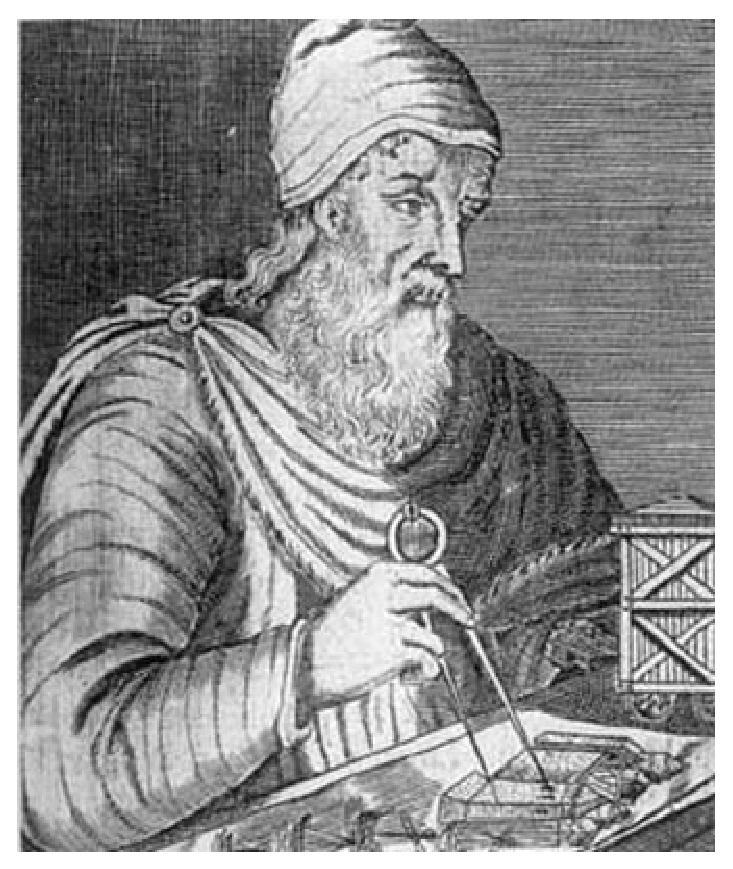
\includegraphics[width=2.5cm]{Nombres_et_calculs_did/Images/Num3_cours_Euclide}
\end{minipage}

\begin{definition}
   Effectuer une division euclidienne d'un {\bf dividende} par un {\bf diviseur}, c'est trouver deux entiers appelés {\bf quotient} et {\bf reste} tels que : \\
   \hspace*{1cm} \og dividende $=$ (diviseur $\times$ quotient) $+$ reste \fg \qquad avec \qquad reste $<$ diviseur.
\end{definition}

\begin{exemple}[0.45]
   Avec une bouteille de \ucl{150} de jus, combien peut-on remplir de verres de \ucl{8} ? \\
   On peut remplir 18 verres de \ucl{8} et il restera \ucl{6} de jus. \\
   On écrit : $\ucl{150} =8\times\ucl{18}+\ucl{6}$ \medskip
   \correction
      \begin{pspicture}(-2,1)(4,3.2)
         \rput(1,1.7){$\opidiv[voperation=top]{150}{8}$}
         \psline[linecolor=A1]{->}(0.7,2.8)(0.7,2.4)
         \rput(0.7,3){\textcolor{A1}{dividende}}
         \psline[linecolor=A1]{<-}(1.9,2.3)(2.4,2.3)
         \rput[l](2.5,2.3){\textcolor{A1}{diviseur}}
         \psline[linecolor=B1]{<-}(2.2,1.7)(2.7,1.7)
         \rput[l](2.8,1.7){\textcolor{B1}{quotient}}
         \psline[linecolor=B1]{<-}(1.4,1.2)(1.9,1.2)
         \rput[l](2,1.2){\textcolor{B1}{reste}}
      \end{pspicture}
\end{exemple}

\begin{definition}
   Effectuer la division décimale d'un {\bf dividende} par un {\bf diviseur}, c'est calculer la valeur exacte ou une valeur approchée du {\bf quotient} \og dividende $\div$ diviseur \fg.
\end{definition}

\begin{exemple}[0.45]
   On achète 8 CD de même prix pour \ueuro{150}. \\ 
   Quel est le prix d'un CD ? \\
   Un CD vaut \ueuro{18,75}. \\
   On écrit : $\ueuro{150} =8\times\ueuro{18,75}$ \medskip
   \correction
      \begin{pspicture}(-2.5,0)(4,2)
         \rput(1,1.2){\opdiv[decimalsepsymbol={,}]{150}{8}}
      \end{pspicture}
\end{exemple}

\bigskip


{\renewcommand{\StringDOCUMENTATION}{Savoirs et savoir-faire pour s'engager dans la division euclidienne}
\begin{documentation}
\begin{enumerate}
   \item Maîtrise des deux sens de la division et des unités de mesure : 
   \begin{itemize}
      \item la division quotition (groupements), c'est la recherche de \og combien de parts ? \fg. \\
      La division se fait entre deux grandeurs identiques.
      \item la division partition (partage), c'est la recherche de la valeur d'une part. \\
      La division se fait entre deux grandeurs différentes.
   \end{itemize}
   \item Maîtrise des tables de multiplication. \\
    Ce qui englobe la recherche de \og Dans 59 combien de fois 7 ? \fg, qui n'est pas directement dans la table de multiplication par 7. \\ [-8mm]
\end{enumerate}
\end{documentation}}

\begin{exemple*1}
   Avec les nombres 21 et 6, on peut proposer les deux sens de la division : \\ [1mm]
   \begin{minipage}{6.5cm}
      {\it J'ai 21 bonbons, combien puis-je faire de paquets de 6 bonbons ?} \\ [1mm]
      Si l'élève veut modéliser la situation, il va faire des paquets de 6 bonbons jusqu'à épuiser les 21 bonbons : \\
      \begin{pspicture}(0,-0.6)(6,2.75)
         \multido{\r=0.5+0.8}{6}{\rput(\r,2.25){
\includegraphics[width=7mm]{Nombres_et_calculs_did/Images/Num3_cours_bonbon}}}
         \rput[l](5,2.25){\footnotesize 6 bonbons}
         \multido{\r=0.5+0.8}{6}{\rput(\r,1.5){
\includegraphics[width=7mm]{Nombres_et_calculs_did/Images/Num3_cours_bonbon}}}
         \rput[l](5,1.5){\footnotesize 12 bonbons}
         \multido{\r=0.5+0.8}{6}{\rput(\r,0.75){
\includegraphics[width=7mm]{Nombres_et_calculs_did/Images/Num3_cours_bonbon}}}
         \rput[l](5,0.75){\footnotesize 18 bonbons}
         \multido{\r=0.5+0.8}{3}{\rput(\r,0){
\includegraphics[width=7mm]{Nombres_et_calculs_did/Images/Num3_cours_bonbon}}}
         \rput[l](2.7,0){\footnotesize 21 bonbons}
      \end{pspicture} \\
      Je peux faire 3 paquets de 6 bonbons et il restera 3 bonbons seuls. \\
      21 bonbons = 3 $\times$ 6 bonbons + 3 bonbons. \smallskip
   \end{minipage}
   \qquad
   \begin{minipage}{6.5cm}
      {\it J'ai 21 bonbons à partager entre 6 amis. \\
      Combien chaque ami va-t-il avoir de bonbons ?} \\ [1mm]
      Si l'élève veut modéliser la situation, il va distribuer un par un les bonbons à chaque ami jusqu'à épuiser les 21 bonbons : \\
      \begin{pspicture}(0,0)(6,3.3)
        \rput(1,2.8){
\includegraphics[width=7mm]{Nombres_et_calculs_did/Images/Num3_cours_bonbon}}
        \rput(1.4,2.5){
\includegraphics[width=7mm]{Nombres_et_calculs_did/Images/Num3_cours_bonbon}}
        \rput(0.7,2.2){
\includegraphics[width=7mm]{Nombres_et_calculs_did/Images/Num3_cours_bonbon}}
        \rput(2,-0.2){\rput(1,3){
\includegraphics[width=7mm]{Nombres_et_calculs_did/Images/Num3_cours_bonbon}}
           \rput(1.4,2.7){
\includegraphics[width=7mm]{Nombres_et_calculs_did/Images/Num3_cours_bonbon}}
           \rput(0.7,2.4){
\includegraphics[width=7mm]{Nombres_et_calculs_did/Images/Num3_cours_bonbon}}}
        \rput(4,-0.2){\rput(1,3){
\includegraphics[width=7mm]{Nombres_et_calculs_did/Images/Num3_cours_bonbon}}
           \rput(1.4,2.7){
\includegraphics[width=7mm]{Nombres_et_calculs_did/Images/Num3_cours_bonbon}}
           \rput(0.7,2.4){
\includegraphics[width=7mm]{Nombres_et_calculs_did/Images/Num3_cours_bonbon}}}
        \rput(0,-1.5){\rput(1,3){
\includegraphics[width=7mm]{Nombres_et_calculs_did/Images/Num3_cours_bonbon}}
           \rput(1.4,2.7){
\includegraphics[width=7mm]{Nombres_et_calculs_did/Images/Num3_cours_bonbon}}
           \rput(0.7,2.4){
\includegraphics[width=7mm]{Nombres_et_calculs_did/Images/Num3_cours_bonbon}}}
        \rput(2,-1.5){\rput(1,3){
\includegraphics[width=7mm]{Nombres_et_calculs_did/Images/Num3_cours_bonbon}}
           \rput(1.4,2.7){
\includegraphics[width=7mm]{Nombres_et_calculs_did/Images/Num3_cours_bonbon}}
           \rput(0.7,2.4){
\includegraphics[width=7mm]{Nombres_et_calculs_did/Images/Num3_cours_bonbon}}}
        \rput(4,-1.5){\rput(1,3){
\includegraphics[width=7mm]{Nombres_et_calculs_did/Images/Num3_cours_bonbon}}
           \rput(1.4,2.7){
\includegraphics[width=7mm]{Nombres_et_calculs_did/Images/Num3_cours_bonbon}}
           \rput(0.7,2.4){
\includegraphics[width=7mm]{Nombres_et_calculs_did/Images/Num3_cours_bonbon}}}
        \multido{\r=0.5+0.8}{3}{\rput(\r,0.2){
\includegraphics[width=7mm]{Nombres_et_calculs_did/Images/Num3_cours_bonbon}}}    
      \end{pspicture} \\
      Je peux donner 3 bonbons à chacun de mes 6  amis et il restera 3 bonbons seuls. \\
      21 bonbons = 6 $\times$ 3 bonbons + 3 bonbons. \smallskip
   \end{minipage}
\end{exemple*1}

\medskip

À partir de là, plusieurs étapes peuvent être suggérées. Un temps préalable suffisant doit être consacré au calcul réfléchi de quotients et de restes. La seconde étape vers la technique peut consister à effectuer des divisions par un nombre à un chiffre, avant de travailler sur des divisions plus complexes, tout en limitant le niveau de difficulté. Dans toutes les circonstances, trois recommandations peuvent être faites : \\
   \hspace*{2mm} -- commencer le calcul par une estimation du nombre de chiffres du quotient ; \\
   \hspace*{2mm} -- s'autoriser à poser des produits annexes, à la suite d'une première estimation du nombre cherché dans le quotient (la production de la totalité de \og la table du diviseur \fg{} ne doit pas être encouragée) ; \\
   \hspace*{2mm} -- encourager la pose effective des soustractions (sans interdire aux élèves qui le souhaitent de s'en dispenser). \smallskip

Deux techniques s'affrontent : celle de la division avec soustractions partielles  posées, et celle sans. Si l'on ne pose pas les soustractions partielles, les élèves doivent calculer mentalement les résultats intermédiaires ce qui est difficile, surtout en cas de retenues ! Dans un premier temps, on peut également utiliser la soustraction comportant des résultats intermédiaires reprenant à chaque étape la totalité du dividende.

\begin{exemple*1}
   Division euclidienne de 557 par 3 selon trois méthodes : \\ [2mm]
   \begin{tabular}{p{0.75cm}p{3.75cm}p{0.25cm}p{3.25cm}p{0.75cm}p{3.75cm}}
      &
      $\opidiv[displayintermediary=all,voperation=top]{557}{3}$ 
      \rput(-1.61,-0.38){0\;0}
      \psline[linewidth=0.16mm](-1.9,-0.593)(-1.3,-0.593)
      \psframe[fillstyle=solid,fillcolor=white,linecolor=white](-0.7,-0.52)(-0.1,-0.2)
      \rput(-0.45,-0.37){0\;0}
      \rput(-1.45,-0.88){7}
      \rput(-0.6,-0.88){+\;8\;0}
      \rput(-1.45,-1.38){0}
      \psline[linewidth=0.16mm](-1.63,-1.605)(-1.3,-1.605)
      \rput(-0.61,-1.4){+\quad5}
      \psline[linewidth=0.16mm](-1,-1.605)(-0.1,-1.605)
      \rput(-0.60,-1.89){1\;8\;5}
      &&
      $\opidiv[displayintermediary=all,voperation=top]{557}{3}$
      &&
      $\opidiv[voperation=top]{557}{3}$
      \\
      \multicolumn{2}{c}{$+$ \small sens à l'opération, erreur rattrapable}
      &
      \multicolumn{2}{c}{$+$ \small technique usuelle}
      &
      \multicolumn{2}{c}{$+$ \small gain de temps et de place}
      \\
      \multicolumn{2}{c}{$-$ \small lourdeur de l'écriture}
      &\multicolumn{2}{c}{$-$ \small compréhension}
      &\multicolumn{2}{c}{$-$ \small source d'erreurs, surcharge cognitive}
      \\ [2mm]
   \end{tabular}
   À la suite, on peut écrire l'équation qui caractérise la division euclidienne : $557 =3\times185+2$.
\end{exemple*1}

\medskip

Pour introduire l'écriture en potence, on peut utiliser un matériel de numération (faux billets/pièces, multibase\dots) afin de manipuler les nombres sur une situation concrète et de faire le lien avec l'écriture de la division euclidienne.

\begin{exemple*1}
   On peut proposer la situation suivante issue d'une animation pédagogique sur la division au CE2 aux Andelys en 2011 : \\
   {\it Le chef des pirates veut partager 557 pièces d’or en 3 parts égales. Comment peut-il faire ?}
\end{exemple*1}

\bigskip

Avec le matériel mutibase, les élèves doivent partager une certaine quantité d'or. On les laissera manipuler et organiser leur recherche comme il le le souhaitent. À l'issue de la mise en commun, on décide de commencer par les centaines et d'introduire la notation classique français avec la potence.

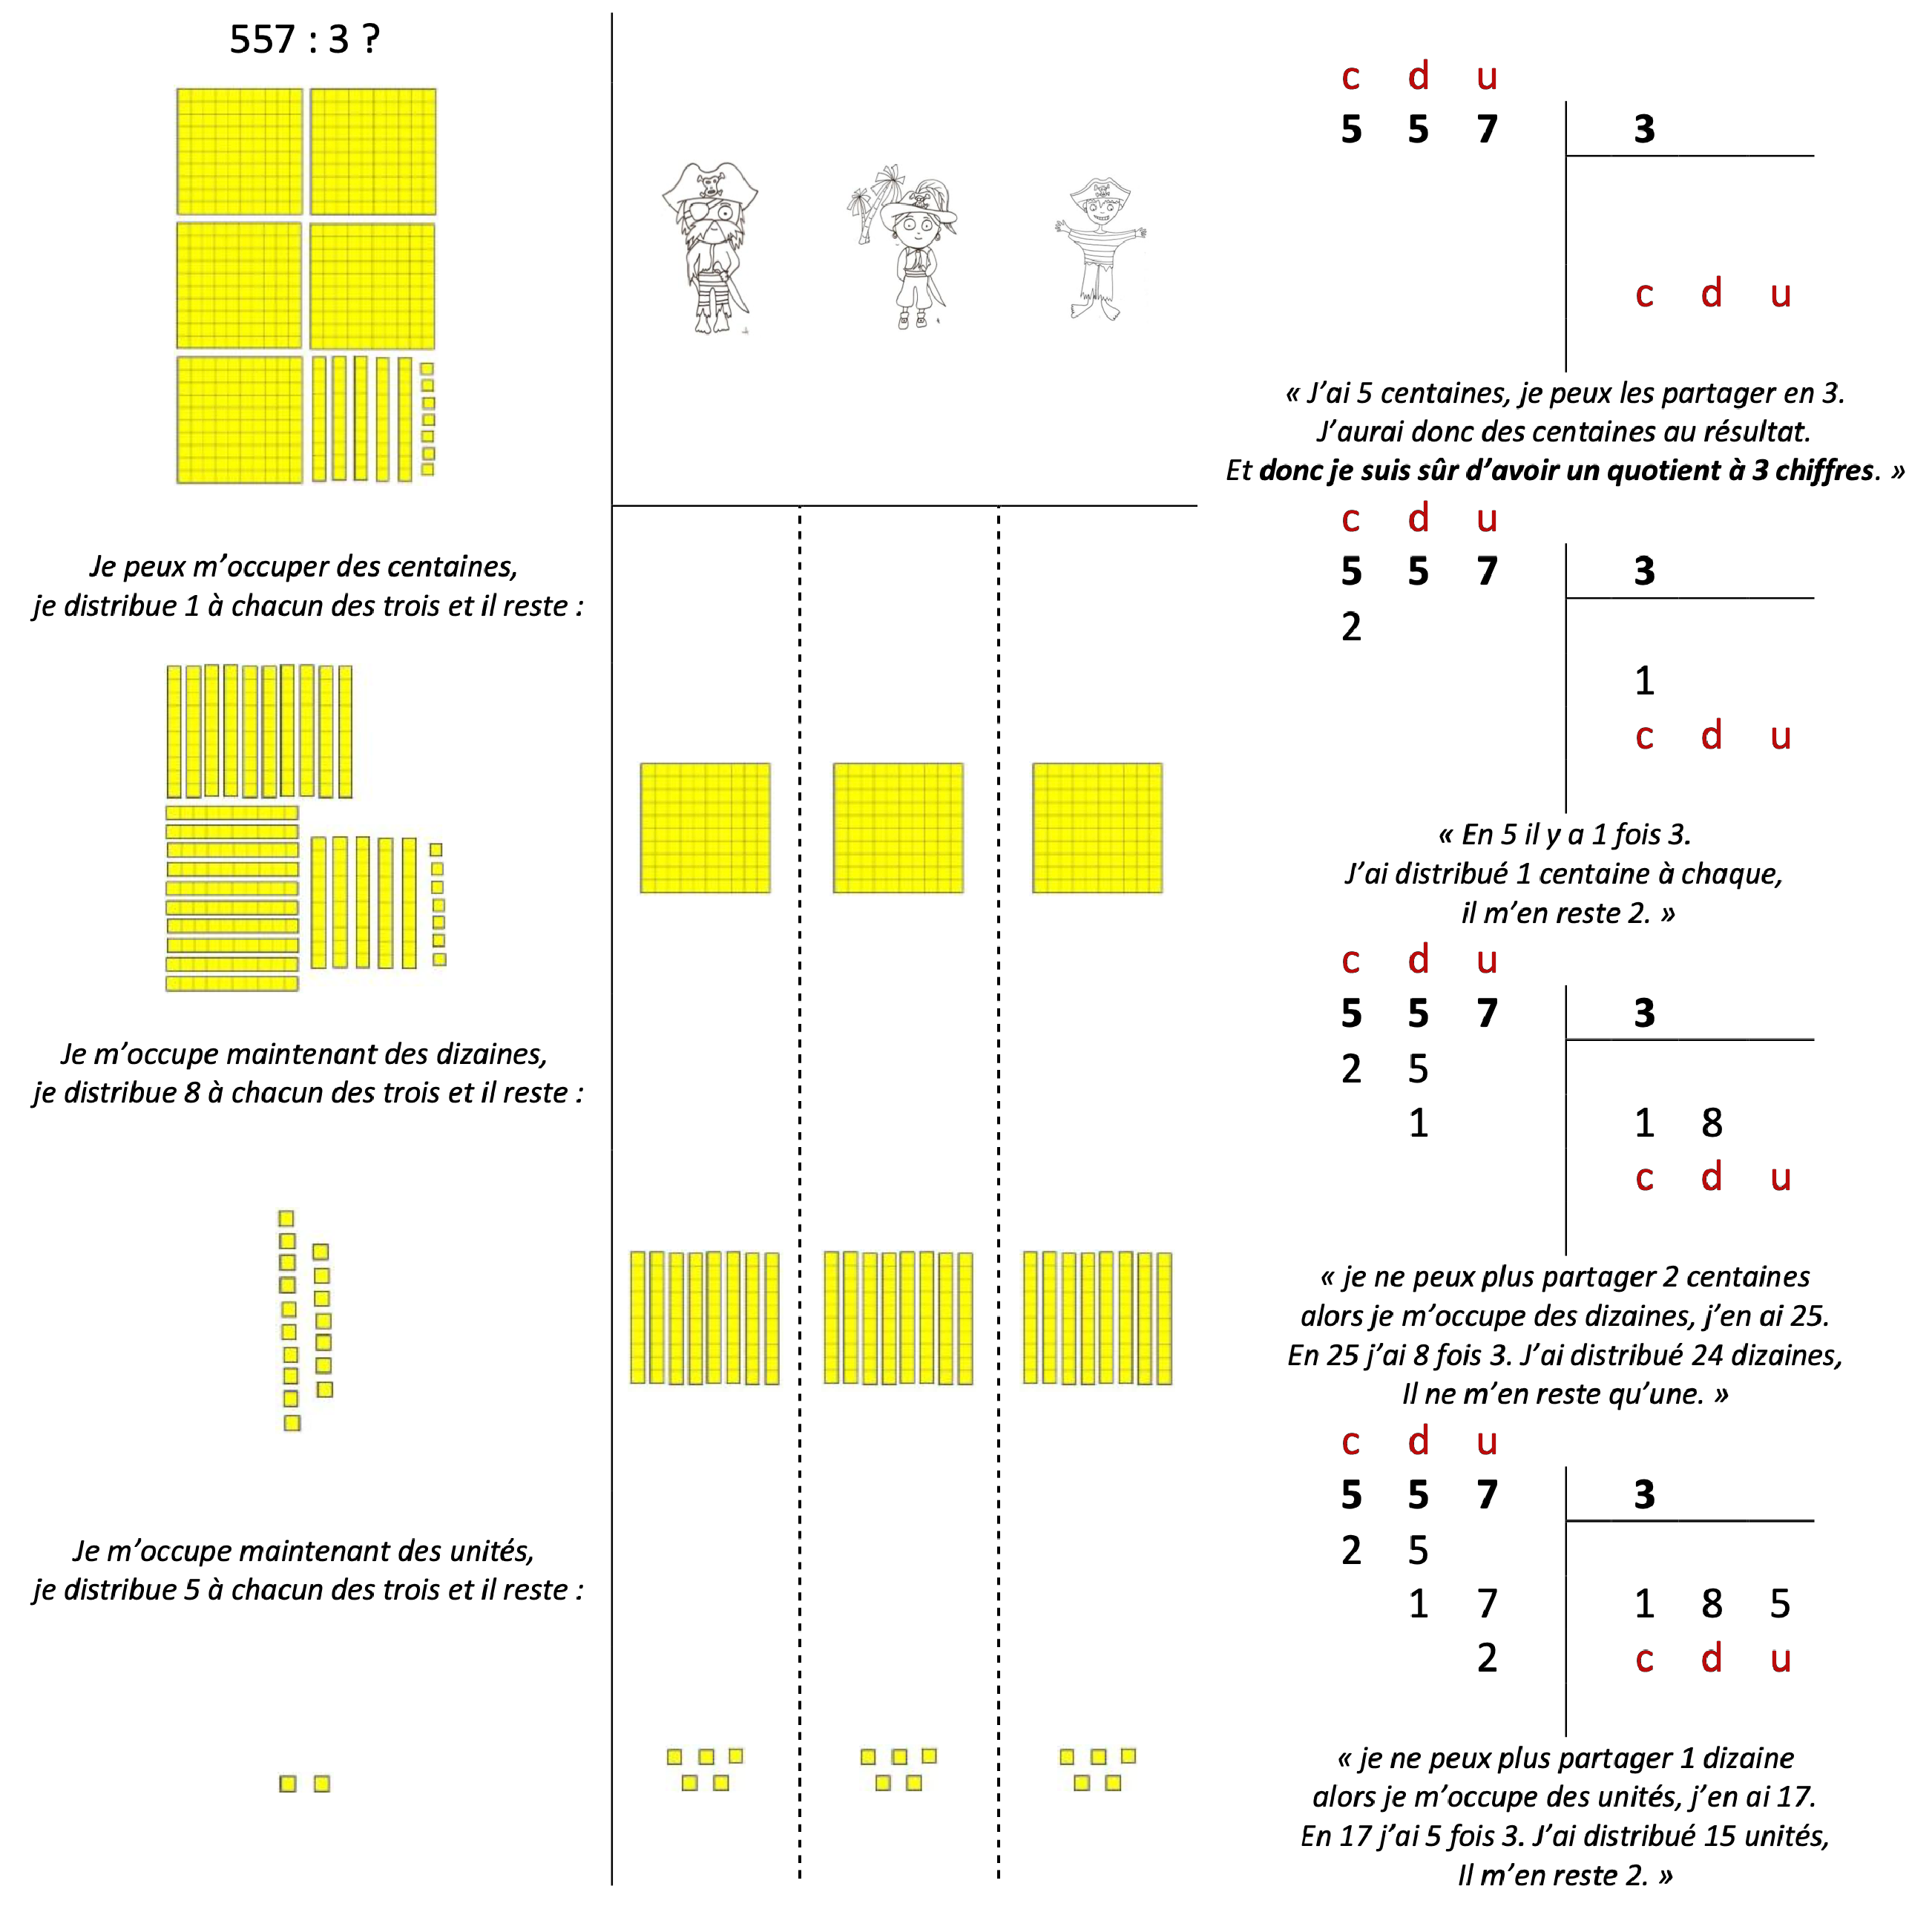
\includegraphics[width=16.4cm]{Nombres_et_calculs_did/Images/Num3_cours_pirates}

{\renewcommand{\StringDOCUMENTATION}{Difficultés rencontrées par les élèves}
\begin{documentation}
   \begin{itemize}
      \item Les calculs s'effectuent \og de gauche à droite \fg.
      \item Nécessité d'effectuer simultanément des divisions, multiplications et soustractions.
      \item Les chiffres écrits successivement pour constituer le quotient sont le résultat d'une approximation qui peut conduire à essayer un chiffre erroné, donc provisoire. \\ [-8mm]
   \end{itemize}
\end{documentation}}
   

\subsection{Procédures utilisées pour résoudre des problèmes multiplicatifs} %%%

Cette partie s'inspire du \og Hatier concours, Professeur des écoles, Admissibilité, Mathématique, Tome 2 \fg{}, {\it Roland Charnay, Michel Mante} [cha13-2]. \\

{\bf Problèmes \og de multiplication \fg}. On considère l'exemple suivant :

\smallskip

\begin{cadre}[B2][J2]
   {\bf La directrice d'une école maternelle a acheté \bm{$n$} boites de \bm{$p$} crayons. Combien a-t-elle acheté de crayons ?}
\end{cadre}

\smallskip

On peut utiliser (au moins) trois types de procédures pour effectuer le calcul :
{\renewcommand{\StringDOCUMENTATION}{Les procédures}
\begin{documentation}
\begin{enumerate}
   \item une procédure de type dessin ou schéma ;
   \item une procédure de type calcul additif ;
   \item une procédure de type calcul multiplicatif. 
\end{enumerate}
\ \\ [-12mm]
\end{documentation}}

\bigskip

Résumons dans un tableau ces procédures en fonction des nombres $n$ et $p$ :

{\renewcommand{\arraystretch}{1.7}{
\begin{CLtableau}{\linewidth}{4}{c}
   \hline
   &
   $n$ et $p$ sont petits \newline
   {\it ex : 4 boites de 6 crayons}
   &
   $n$ est petit et $p$ est grand \newline
   {\it ex : 4 boites de 24 crayons}
   &
   $n$ et $p$ sont grands \newline
   {\it ex : 36 boites de 24 crayons} \\
   \hline   
   1.
   &
   L'élève représente les 4 boites de 6 crayons : \newline
   \newline
   \fbox{|\!|\!|\!|\!|\!| \; |\!|\!|\!|\!|\!| \; |\!|\!|\!|\!|\!|  \; |\!|\!|\!|\!|\!|} \newline
   \newline
   puis les dénombre un par un ou six par six.
   &
   Possible, mais procédure très coûteuse !
   &
   Procédure inutilisable dans ce cas. \\
   \hline
   2.
   &
   $6+6+6+6=24$ \newline
   ou \newline
   \og 6 \, ; \, 12 \, ; \, 18 \, ; \, 24 \fg.
   &
   Efficace à condition de savoir calculer des sommes de nombres à deux chiffres et plus, et d'organiser au mieux ses calculs : \newline
  \psset{nodesep=1mm}
     $\hspace*{0.5cm} \rnode{a}{24}\,+\,\rnode{b}{24}\,+\,\rnode{c}{24}\,+\,\rnode{d}{24}$ \newline \newline     
     \hspace*{0.7cm} $\rnode{g}{48} \hspace*{0.4cm} + \hspace*{0.5cm} \rnode{h}{48}$ \newline \newline
      \hspace*{0.1cm} $\rnode{j}{96}$
      \ncline{a}{g}
      \ncline{b}{g}
      \ncline{c}{h}
      \ncline{d}{h}
      \ncline{g}{j}
      \ncline{h}{j}    
   &
   Procédure très longue. \\
   \hline  
   3.
   &
   Calcul mental de $4\times6$ à l'aide des tables de multiplication.
   &
   Très efficace si on connait la procédure experte : \newline
   \newline
   $\opmul{24}{4}$
   &
   Procédure experte requise ici. \newline
   \newline
   $\opmul{24}{36}$
   \\
   \hline
\end{CLtableau}}}

\newpage


{\bf Problèmes \og de division \fg}. On considère l'exemple suivant :
On considère l'exemple suivant :

\begin{cadre}[B2][J2]
   {\bf On range 67 oeufs dans des boîtes de 12. Combien de boîtes peut-on remplir ?}
\end{cadre}

{\renewcommand{\arraystretch}{1.5}{
   \begin{Ltableau}{1\linewidth}{2}{m{6.2cm}|m{9.78cm}}
      \hline
         \multicolumn{2}{|c|}{Procédure de type dessin ou schéma.} \\
      \hline
      Dessin figuratif \newline
      \begin{pspicture}(2,1.1)
         \psframe(-0.05,-0.1)(1.95,0.9)
         \psellipse(0.2,0.2)(0.1,0.15)
         \psellipse(0.5,0.2)(0.1,0.15)
         \psellipse(0.8,0.2)(0.1,0.15)
         \psellipse(1.1,0.2)(0.1,0.15)
         \psellipse(1.4,0.2)(0.1,0.15)
         \psellipse(1.7,0.2)(0.1,0.15)
         \psellipse(0.2,0.6)(0.1,0.15)
         \psellipse(0.5,0.6)(0.1,0.15)
         \psellipse(0.8,0.6)(0.1,0.15)
         \psellipse(1.1,0.6)(0.1,0.15)
         \psellipse(1.4,0.6)(0.1,0.15)
         \psellipse(1.7,0.6)(0.1,0.15)
      \end{pspicture}
      \begin{pspicture}(2,1.1)
         \psframe(-0.05,-0.1)(1.95,0.9)
         \psellipse(0.2,0.2)(0.1,0.15)
         \psellipse(0.5,0.2)(0.1,0.15)
         \psellipse(0.8,0.2)(0.1,0.15)
         \psellipse(1.1,0.2)(0.1,0.15)
         \psellipse(1.4,0.2)(0.1,0.15)
         \psellipse(1.7,0.2)(0.1,0.15)
         \psellipse(0.2,0.6)(0.1,0.15)
         \psellipse(0.5,0.6)(0.1,0.15)
         \psellipse(0.8,0.6)(0.1,0.15)
         \psellipse(1.1,0.6)(0.1,0.15)
         \psellipse(1.4,0.6)(0.1,0.15)
         \psellipse(1.7,0.6)(0.1,0.15)
      \end{pspicture}
      \begin{pspicture}(2,1.1)
         \psframe(-0.05,-0.1)(1.95,0.9)
         \psellipse(0.2,0.2)(0.1,0.15)
         \psellipse(0.5,0.2)(0.1,0.15)
         \psellipse(0.8,0.2)(0.1,0.15)
         \psellipse(1.1,0.2)(0.1,0.15)
         \psellipse(1.4,0.2)(0.1,0.15)
         \psellipse(1.7,0.2)(0.1,0.15)
         \psellipse(0.2,0.6)(0.1,0.15)
         \psellipse(0.5,0.6)(0.1,0.15)
         \psellipse(0.8,0.6)(0.1,0.15)
         \psellipse(1.1,0.6)(0.1,0.15)
         \psellipse(1.4,0.6)(0.1,0.15)
         \psellipse(1.7,0.6)(0.1,0.15)
      \end{pspicture} \newline
      \begin{pspicture}(2,1.1)
         \psframe(-0.05,-0.1)(1.95,0.9)
         \psellipse(0.2,0.2)(0.1,0.15)
         \psellipse(0.5,0.2)(0.1,0.15)
         \psellipse(0.8,0.2)(0.1,0.15)
         \psellipse(1.1,0.2)(0.1,0.15)
         \psellipse(1.4,0.2)(0.1,0.15)
         \psellipse(1.7,0.2)(0.1,0.15)
         \psellipse(0.2,0.6)(0.1,0.15)
         \psellipse(0.5,0.6)(0.1,0.15)
         \psellipse(0.8,0.6)(0.1,0.15)
         \psellipse(1.1,0.6)(0.1,0.15)
         \psellipse(1.4,0.6)(0.1,0.15)
         \psellipse(1.7,0.6)(0.1,0.15)
      \end{pspicture}
      \begin{pspicture}(2,1.1)
         \psframe(-0.05,-0.1)(1.95,0.9)
         \psellipse(0.2,0.2)(0.1,0.15)
         \psellipse(0.5,0.2)(0.1,0.15)
         \psellipse(0.8,0.2)(0.1,0.15)
         \psellipse(1.1,0.2)(0.1,0.15)
         \psellipse(1.4,0.2)(0.1,0.15)
         \psellipse(1.7,0.2)(0.1,0.15)
         \psellipse(0.2,0.6)(0.1,0.15)
         \psellipse(0.5,0.6)(0.1,0.15)
         \psellipse(0.8,0.6)(0.1,0.15)
         \psellipse(1.1,0.6)(0.1,0.15)
         \psellipse(1.4,0.6)(0.1,0.15)
         \psellipse(1.7,0.6)(0.1,0.15)
      \end{pspicture}
      \begin{pspicture}(2,1.1)
         \psellipse(0.2,0.2)(0.1,0.15)        
         \psellipse(0.2,0.6)(0.1,0.15)
         \psellipse(0.5,0.6)(0.1,0.15)
         \psellipse(0.8,0.6)(0.1,0.15)
         \psellipse(1.1,0.6)(0.1,0.15)
         \psellipse(1.4,0.6)(0.1,0.15)
         \psellipse(1.7,0.6)(0.1,0.15)
      \end{pspicture}
       \newline
      Dessin schématisé \newline
      \fbox{\huge{12}} \, \fbox{\huge{12}} \, \fbox{\huge{12}} \, \fbox{\huge{12}} \, \fbox{\huge{12}} \, \huge{7} 
      &
      Ces procédures deviennent très vite peu économiques et difficiles à gérer dès que les nombres sont grands. \newline
      Il s'agit souvent de procédures d'entrée dans le problème qui permettent à l'élève de comprendre la situation et d'imaginer une autre procédure plus rapide. \\
      \hline  
   \end{Ltableau}}}
   
{\renewcommand{\arraystretch}{1.7}{
   \begin{Ltableau}{1\linewidth}{2}{m{6.2cm}|m{9.78cm}}
      \hline
         \multicolumn{2}{|c|}{Procédure progressive basée sur l'addition ou la soustraction} \\
      \hline    
      Additions \og pas à pas \fg{} : \newline
      $12 +12 = 24 + 12 = 36 + 12 = 48 +12 = 60 + 7 = 67$ \newline
      ou \newline
      $12 + 12 + 12 = 36$ \newline
      $36+36 =72$ \newline
      $12+12 =24$ \newline
      $36+24 =60$ \newline
      $60+7 =67$
      &
      La première suite d'égalités est correcte du point de vue de la démarche : l'élève simule le remplissage des boites une à une en faisant le bilan des \oe ufs utilisés après chaque boite remplie. Cependant, le statut du signe \og = \fg{} ne semble pas tout à fait compris puisque les égalités ne sont pas vraies dans leur globalité. \newline
      La seconde démarche est comparable, mais l'élève fait des bilans partiels et réutilise ses calculs antérieurs. \newline
      Une difficulté est de retrouver à la fin le nombre de fois que l'on a utilisé \og 12 \fg. \\
      \hdashline
      Soustractions \og pas à pas \og \newline
      $67-12 =55$ \newline
      $55-12 =43$ \newline
      $43-12 =31$ \newline
      $31-12 =19$ \newline
      $19-12 =7$
      &
      L'élève s'intéresse aux \oe ufs restants à mettre en boite plutôt qu'aux \oe ufs utilisés. \newline
      Ces procédures deviennent vite coûteuses avec des nombres assez grands. \newline
      Certains élèves, parvenus à la fin de leurs calculs, ne savent plus comment retrouver le nombre de boîtes (surcharge cognitive). \\
   \hdashline
      Additions et/ou soustractions de multiples du diviseur : \newline
      \hspace*{1cm} $\opadd{36}{36}$ \quad et \quad $\opsub[carrysub=true]{72}{5}$
      &
      Ce sont des améliorations des procédures précédents, l'élève utilisant souvent un résultat obtenu mentalement qui correspond au remplissage de plusieurs boites à la fois. \newline
      La même difficulté que précédemment pour compter le nombre de boites se pose. \\
      \hline
   \end{Ltableau}}}
   
{\renewcommand{\arraystretch}{1.7}{
   \begin{Ltableau}{1\linewidth}{2}{m{6.2cm}|m{9.78cm}}
      \hline
         \multicolumn{2}{|c|}{Procédure de type calcul multiplicatif : l'élève cherche à résoudre une équation du type $12\times\dots=67$} \\
      \hline Pose de la multiplication à trous : \newline
      \hspace*{1.8cm} \begin{tabular}{C{0.1}C{0.1}C{0.1}}
      & 1 & 2 \\
      $\times$ & {\Huge .} & {\Huge .}  \\
      \hline
      & 6 & 7 \\
      \end{tabular}
      &
      Procédure délicate lorsque le reste n'est pas nul puisqu'elle n'est pas possible en une seule opération. \\
      \hdashline
      Essais de multiples successifs du diviseur : \newline
      $12\times4 =48$ ; \newline
      $12\times5 =60$ ; \newline
      $12\times6 =72$
      &
      Procédure qui peut être fastidieuse si l'élève a commencé son évaluation avec un nombre trop petit. \newline
      Nécessite ensuite un ajustement pour trouver le bon résultat. \\
      \hdashline
      Essais par approches successives : \newline
      \hspace*{0.5cm} $\opmul{12}{4}$ \qquad $\opmul{12}{8}$ \qquad $\opmul{12}{6}$ \qquad $\opmul{12}{5}$
      &
       L'efficacité de cette procédure dépend à la fois de la qualité de l'approximation effectuée au départ et des ajustements successifs. \\
       \hline
    \end{Ltableau}}}

\bigskip

{\renewcommand{\arraystretch}{1.5}{
   \begin{Ltableau}{1\linewidth}{2}{m{6.2cm}|m{9.78cm}}
      \hline
         \multicolumn{2}{|c|}{Procédure mixte utilisant à la fois la multiplication et la soustraction} \\
      \hline   
     Calculs partiels \og au hasard \fg{} : \newline
     \hspace*{1.5cm} $\opmul[voperation=top]{12}{3}$ \qquad $\opsub[voperation=top]{67}{36}$ \newline \newline
      puis \newline
      \hspace*{1.5cm} $\opmul[voperation=top]{12}{2}$ \qquad $\opsub[voperation=top]{31}{24}$ \newline
     &
     L'élève fait un essai de multiple, calcule l'écart entre ce produit et le dividende puis recommence avec l'écart. \newline
    L'élève pourra également commencer par utiliser des multiples de 10, 100 si le nombre est grand. \\
    \hline
    \end{Ltableau}}}

\bigskip
    
{\renewcommand{\arraystretch}{1.5}{
   \begin{Ltableau}{1\linewidth}{2}{m{6.2cm}|m{9.78cm}}
      \hline
         \multicolumn{2}{|c|}{Procédure experte de la division euclidienne} \\
      \hline
      Calcul de la division de la euclidienne de 67 par 12 : \newline
      \hspace*{2cm} $\opidiv[displayintermediary=all]{67}{12}$ \newline
      ou \newline      
      utilisation d'une calculatrice.
      &
      Procédure experte dont relève le problème posé. Le but étant d'amener progressivement l'élève à utiliser cette procédure. \\
      \hline
   \end{Ltableau}}}

\bigskip

Pour les problèmes qui se résolvent par une multiplication ou une division, il existe de multiples variables didactiques, comme par exemple : le {\bf type de problèmes} (une, plusieurs ou composition de grandeurs) ; le type de {\bf nombres utilisés} (nombre entiers et/ou décimaux) ; la {\bf taille des nombres} en jeu ; les {\bf outils de calcul} disponibles ou non (calculatrice, abaque) ; le {\bf contexte} (plus ou moins familier) ; ma manière dont l'{\bf énoncé} est formulé (compréhensible ou complexe, présence de mots inducteurs) ; existence ou non d'un {\bf reste} non nul pour la division\dots


%%%%%%%%%%%%%%%%%%%%%%%%%%%%%
%%%%%%%%%%%%%%%%%%%%%%%%%%%%%
\activites

\textcolor{G1}{Documents 1 à 4 issus du livre \og {\it Leçon, le manuel complet pour réussi l'oral} \fg, CRPE 2022, Vuibert.} \\

{\bf\uline{Consigne candidat}} : À partir du sujet et du dossier proposés par le jury, vous concevrez la mise en œuvre d'une séance d'enseignement à l'école primaire dans chacune des deux disciplines français et mathématiques. Vous présenterez successivement les composantes pédagogiques et didactiques de chaque séance et son déroulement. \\

{\bf\uline{Sujet}} : La soustraction posée. \\

{\bf\uline{Contexte de la séance d'enseignement}} : \\
   \hspace*{5mm} -- cycle d'enseignement : cycle 2 ; \\
   \hspace*{5mm} -- niveau de la classe : CE1 ; \\
   \hspace*{5mm} -- positionnement de la séance de mathématiques : \\
      \hspace*{10mm} -- période : non précisé ; \\
      \hspace*{10mm} -- séquence dans laquelle elle s'insère : technique de calcul posé pour la soustraction. \\ [10mm]

{\bf\uline{Documents fournis au candidat}} : \\

{\bf\uline{Document 1}} : Extrait des repères annuels de progression, cycle 2. Ministère de l'Éducation nationale, de la Jeunesse et des Sports.

\begin{center}
   \textsf{
      \begin{tabular}{|p{5cm}|p{5cm}|p{5cm}|}
         \arrayrulecolor{teal}
         \hline
         \hspace*{2.3cm} \textcolor{teal}{\bf CP} & \hspace*{2.3cm} \textcolor{teal}{\bf CE1} & \hspace*{2.3cm} \textcolor{teal}{\bf CE2} \\
         \hline
         \multicolumn{3}{|c|}{\textcolor{teal}{Calcul (suite)}} \\
         \hline
         \multicolumn{3}{|p{16cm}|}{Les {\bf procédures} à mémoriser dans le cadre du calcul posé. \newline
         Les opérations posées permettent l’obtention de résultats notamment lorsque le calcul mental ou écrit en ligne atteint ses limites. Leur apprentissage est aussi un moyen de renforcer la compréhension du système décimal de position et de consolider la mémorisation des relations numériques élémentaires. Il a donc lieu lorsque les élèves se sont approprié des stratégies de calcul basées sur des décompositions/recompositions liées à la numération décimale, souvent utilisées également en calcul mental ou écrit.} \\
         \hline
         Les élèves enrichissent d’abord la mémorisation de faits numériques et de procédures. Au plus tard en {\bf période 4}, les élèves apprennent à poser les additions en colonnes avec des nombres de deux chiffres.
         &
         Dès le {\bf début de l’année}, les élèves consolident la maîtrise de l'addition avec des nombres plus grands et avec des nombres de taille différente. \newline
         Ils continuent à enrichir la mémorisation de faits numériques et de procédures. Au plus tard en {\bf période 3}, les élèves apprennent une technique de calcul posé pour la soustraction.
         &
         Dès le {\bf début de l’année}, les élèves consolident la maîtrise de la technique de la soustraction apprise en CE1. \newline
         Ils apprennent et entretiennent {\bf tout au long de l’année} une technique de calcul posé pour la multiplication, tout d’abord en multipliant un nombre à deux chiffres par un nombre à un chiffre puis avec des nombres plus grands. \\
         \hline
         \multicolumn{3}{|p{16cm}|}{Les techniques de calcul posé sont communes à toutes les classes, elles sont ritualisées avec les mêmes formes et les mêmes mots. Ce choix doit être poursuivi au cycle 3.} \\
         \hline
      \end{tabular}
   }
\end{center}

\bigskip


{\bf\uline{Document 2}} : Extrait de la note de service n°2018-051 du 25-4-2018 \og {\it Enseignement du calcul : un enjeu majeur pour la maîtrise des principaux éléments de mathématiques à l'école primaire} \fg.

\begin{center}
   \begin{minipage}{15cm}
         \textsf{{\bf LE CACLUL POSÉ} \\
         Le calcul posé repose sur la connaissance de faits numériques (tables) et sur celle d'algorithmes qui ne sont véritablement opératoires que s'ils sont parfaitement maîtrisés.
Ainsi, les quatre algorithmes opératoires (pour l'addition, la soustraction, la multiplication, la division) doivent faire l'objet d'un enseignement précis, guidé et normalisé. Au début de l'apprentissage, le rythme doit être suffisamment soutenu afin que l'automaticité - et donc le confort et la sûreté pour l'élève - puissent s'installer. Ensuite, à partir du CE1, la plupart des séances de mathématiques donnent l'occasion aux élèves de poser une ou plusieurs opérations.
Pour autant, une fois les principes de fonctionnement d'un algorithme d'une opération posée acquis par les élèves, le cadre privilégié pour l'entraînement à la mise en œuvre de cet algorithme est celui de la résolution de problèmes. Il faut ainsi éviter la pratique répétée d'exercices techniques sur des temps excessivement longs. Dans le même esprit, on évitera les exercices de calcul d'opérations posées trop longues comme par exemple la multiplication de nombres supérieurs à 1 000 ou la division par des grands nombres.
Pour la soustraction, le choix de l'algorithme (compensation ou cassage de l'unité de numération supérieure) relève de l'équipe d'école. On aura intérêt à conserver le même durant les quatre années concernées (du CE1 au CM2). [...] \\
         La justification mathématique de la pertinence des algorithmes opératoires est d'une difficulté inégale selon l'opération : [...] \\
         -- pour la soustraction, si c'est le choix du cassage de l'unité de numération supérieure qui est fait, [...] le maître doit justifier l'algorithme par l'utilisation de matériel puis l'oralisation ; en revanche, si c'est le choix de la compensation qui est fait, une justification peut être donnée, basée sur des écritures en ligne (75-29 = (75+10) - (29+10), c'est pour cela que l'on dit « 9 ôtés de 5 je ne peux pas, donc je fais 9 ôtés de 15 (ce qui revient à ajouter une dizaine à 75), je pose 6 et je retiens 1 ; 2 et 1 de retenue (ce qui revient à ajouter une dizaine à 29) qui font 3, 3 ôtés de 7 font 4 ») sans qu'il soit demandé à tous les élèves de mémoriser cette explicitation ; [...] \\ [2mm]
         {\bf CALCUL MENTAL, CACLUL EN LIGNE OU CALCUL POSÉ ?} \\
         Il n'y a pas lieu d'opposer les différents modes de calcul. Chacun doit faire l'objet d'un entraînement spécifique. L'élève, lorsqu'il doit produire un résultat, par exemple pour une résolution de problèmes, doit pouvoir choisir le mode de calcul qui lui paraît, à lui, dans cette situation, avec ses connaissances, le plus sûr et/ou le plus rapide et/ou le plus facile.
         }
   \end{minipage}
\end{center}

\bigskip


{\bf\uline{Document 3}} : Extrait d'\og {\it Enseigner les mathématiques à l'école} \fg, Thierry Dias, Magnard 2018, pp. 172-174.

\begin{center}
   \begin{minipage}{16cm}
      \textsf{Nous allons étudier trois techniques, fondées sur trois principes distincts, qui peuvent constituer un bon matériau pour différencier. [...] \\
      {\bf La méthode par \og cassage \fg} \\
      Cette technique est la plus simple à comprendre et elle est utilisée dans certains pays, comme la Suisse et les États-unis. Elle permet en effet de bien comprendre le système des groupements et échanges qui conditionne la numération décimale.} \\ [2mm]
      \begin{minipage}{13cm}
         \textsf{La voici schématisée sur un exemple : 753 $-$ 85. \\
         Avec cette technique, on commence bien sûr par les unités, en constatant immédiatement que la soustraction 3 $-$ 5 n'est pas possible dans l'ensemble des entiers naturels. Pour obtenir davantage d'unités dans le premier terme, on \og casse \fg{} une dizaine (c'est-à-dire que I'on défait un groupement de dix). Des 75 dizaines que nous avions, il en restera donc 74 : on barre le 5 I'on écrit 4 à la place. Maintenant que l'on a 13 unités (10 $+$ 3), on peut soustraire 5 : on effectue 13 $-$ 5 pour trouver 8. C'est le chiffre résultat de la colonne des unités. \medskip}
      \end{minipage}
      \quad
      \begin{minipage}{2.5cm}
               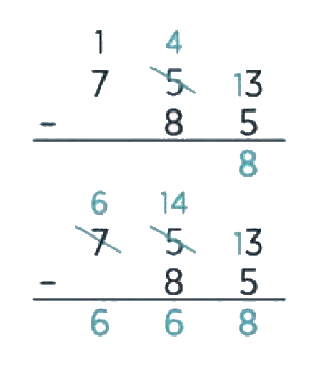
\includegraphics[width=2.5cm]{Nombres_et_calculs_did/Images/Num3_crpe_cassage}
      \end{minipage} \\
      \textsf{On refait ensuite la mème opération, qui consiste à défaire un groupe de cent pour obtenir davantage de dizaines. Cette technique opératoire repose donc sur des réécritures successives du premier terme. Dans les situations où ce nombre comporte plusieurs zéros, la technique devient laborieuse et complexe, car on doit le barrer plusieurs fois [...].}
   \end{minipage}

   \begin{minipage}{16cm}
      \textsf{{\bf La méthode par \og compléments \fg} \\
      Cette technique consiste à transformer la soustraction en une addition à trous. Elle revient donc à utiliser ses connaissances sur l'addition pour les reporter dans un calcul soustractif. Ici, on cherche un nombre qui, ajouté à 85, donne 753.} \\ [1mm]
      \begin{minipage}{13.3cm}
      \textsf{On doit donc aller de 5 à 3 en avançant mais, comme ce n'est pas possible, on va aller de 5 à 13, d'où la retenue que I'on pose ici en bleu. Pour aller de 5 à13, il faut 8. \\
      On continue ainsi : pour aller de 8 $+$ 1 $=$ 9 à 5, ce n'est pas possible ; on va donc de 9 à15, etc.} \smallskip
      \end{minipage}
      \quad
      \begin{minipage}{2.2cm}
         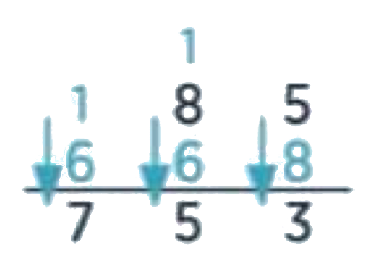
\includegraphics[width=2.2cm]{Nombres_et_calculs_did/Images/Num3_crpe_complement}
      \end{minipage} \\
      \textsf{Cette technique est assez complexe sur le plan sémiotique car se pose alors le problème des retenues. [...] Néanmoins, cette procédure peut se révéler très intéressante si I'on n'essaie pas de la traduire par une écriture en colonnes, mais en appui sur une ligne des nombres. [...] \\ [2mm]    
     {\bf La méthode \og traditionnelle \fg} \\
      Cette technique est la plus courante et c'est probablement celle que vous avez apprise à l'école. Elle repose sur le fait que le résultat d'une soustraction ne change pas si I'on ajoute le même nombre à chacun des termes.} \\ [1mm]
      \begin{minipage}{13cm}
         \textsf{On se retrouve donc avec la même systématique que lors de la première technique : pour enlever 5 à 3, on inscrit \og 13 \fg{} mais, ici, on place la retenue sur la dizaine du nombre juste en dessous du 8. Lorsqu'on ajoute une dizaine à un nombre, on l'ajoute à celui que I'on enlève, et ainsi de suite.} \smallskip
      \end{minipage}
      \quad
      \begin{minipage}{2.5cm}
         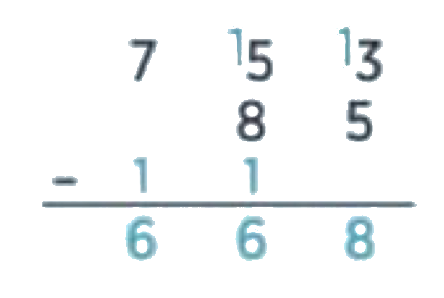
\includegraphics[width=2.5cm]{Nombres_et_calculs_did/Images/Num3_crpe_traditionnelle}
       \end{minipage} \\
      \textsf{Cette technique est très complexe au niveau du sens et provoque un apprentissage très procédural. L'élève l'apprend alors comme un automatisme très symbolique (\og Je dois mettre un petit l ici, et un autre là\dots \fg) sans lui donner de sens. [...] C'est pourtant celle qui est le plus souvent enseignée en France, même si la tendance actuelle est à un basculement vers la première technique.}  
   \end{minipage}
\end{center}

\smallskip


{\bf\uline{Document 4}} : Extraits de manuels scolaires.

\begin{center}
   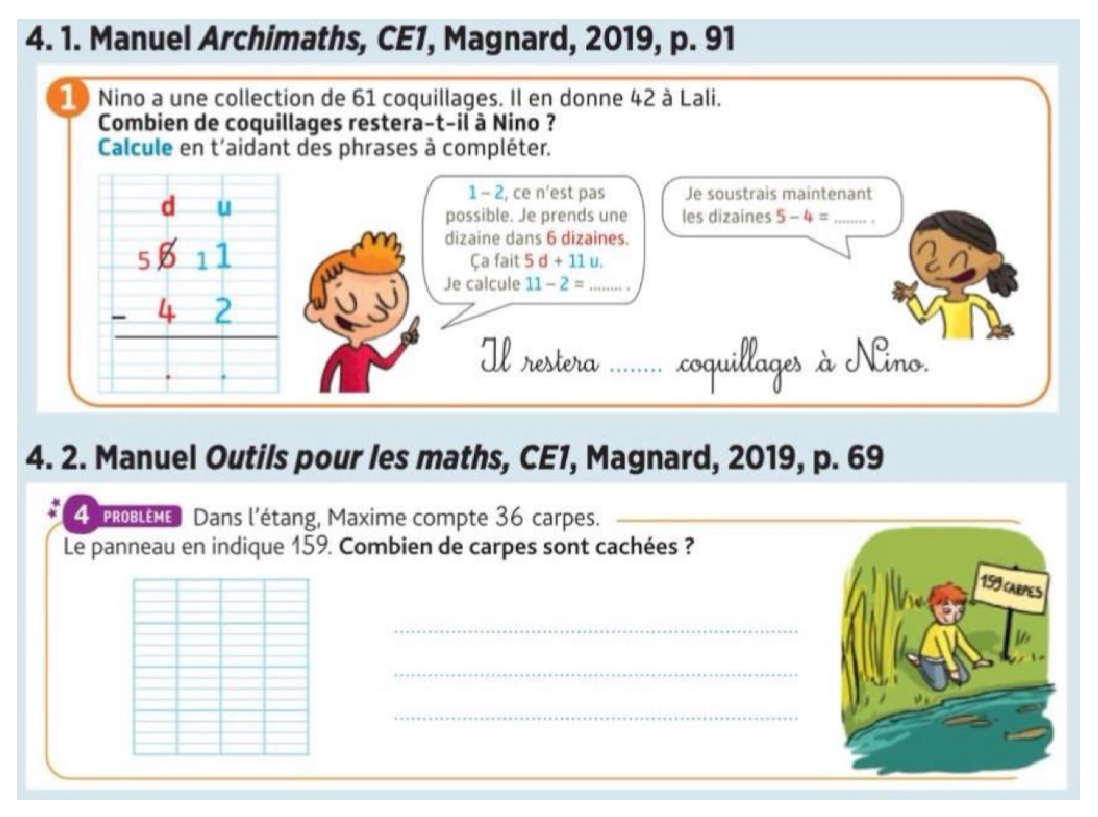
\includegraphics[width=11cm]{Nombres_et_calculs_did/Images/Num3_crpe_archimaths_1} \\
   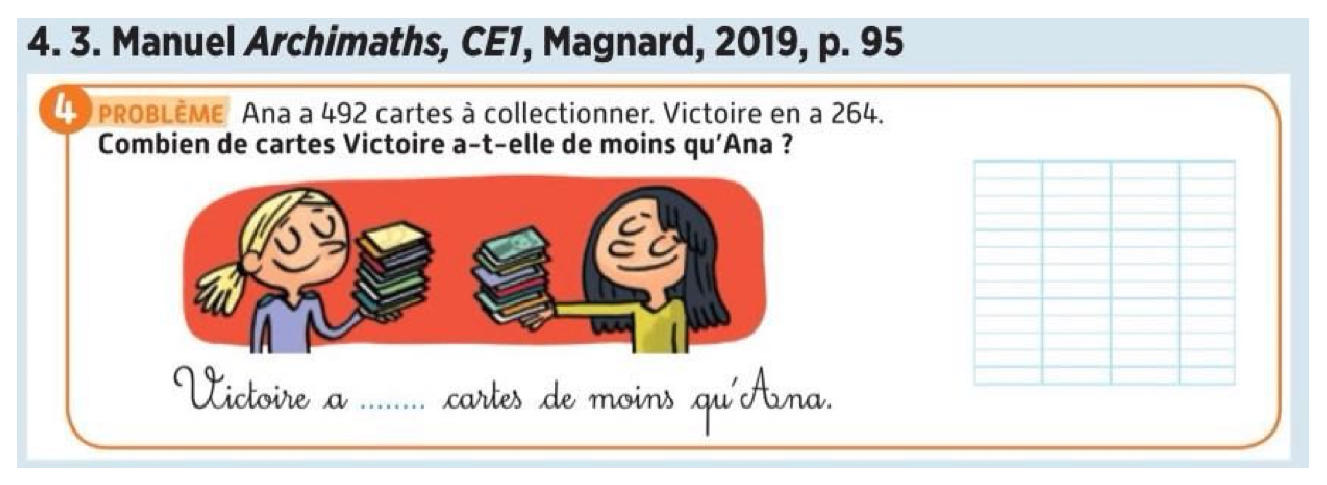
\includegraphics[width=11cm]{Nombres_et_calculs_did/Images/Num3_crpe_archimaths_2}
\end{center}

   
%%%%%%%%%%%%%%%%%%%%%%%%
%%%%%%%%%%%%%%%%%%%%%%%%
\analyses


\begin{exercice}[CRPE 2001 Amiens]
\ \\ [-10mm]
\begin{enumerate}
   \item Classez ces productions issues de l'évaluation CE2 en formulant des hypothèses quant à la nature des erreurs.
   \medskip
   \begin{center}
   \begin{small}
   \begin{tabular}{|*{4}{C{3}|}}
   \hline
   Élève A & Élève B & Élève C & Élève D \\
   \begin{tabular}{*{4}{C{0}}}
      & & & \\
      & \scriptsize 1 & \scriptsize 1 & \\
      & 2 & 3 & 8 \\
      + & 1 & 5 & 9 \\
      + & 3 & 7 & 4 \\
      \hline
      & 7 & 6 & 1 \\
   \end{tabular}
   &
   \begin{tabular}{*{4}{C{0}}}
      & & & \\
      \scriptsize 2 & \scriptsize 6 & \scriptsize 1 & \\
      & 2 & 3 & 8 \\
      + & 1 & 5 & 9 \\
      + & 3 & 7 & 4 \\
      \hline
      & 1 & 1 & 2 \\
   \end{tabular}
   &
   \begin{tabular}{*{4}{C{0}}}
      & & & \\
      & \scriptsize 1 & \scriptsize 2 & \\
      & 2 & 3 & 8 \\
      + & 1 & 5 & 9 \\
      + & 3 & 7 & 4 \\
      \hline
      & 7 & 7 & 1 \\
   \end{tabular}
   &
   \begin{tabular}{*{4}{C{0}}}
      & \scriptsize 1 & & \\
      & \scriptsize 2 & & \\
      & 2 & 3 & 8 \\
      + & 1 & 5 & 9 \\
      + & 3 & 7 & 4 \\
      \hline
      & 9 & 5 & 1 \\
   \end{tabular}
   \\
   & & & \\
   \hline
   Élève E & Élève F & Élève G & Élève H \\
   \begin{tabular}{*{4}{C{0}}}
      & \scriptsize 1 & \scriptsize 2 & \\
      & 2 & 3 & 8 \\
      + & 1 & 5 & 9 \\
      + & 3 & 7 & 4 \\
      \hline
      & 7 & 8 & 1 \\
   \end{tabular}
   &
   \begin{tabular}{*{4}{C{0}}}
      & \scriptsize 1 & \scriptsize 2 & \\
      & 2 & 3 & 8 \\
      + & 1 & 5 & 9 \\
      + & 3 & 7 & 4 \\
      \hline
      & 6 & 5 & 1 \\
   \end{tabular}
   &
   \begin{tabular}{*{4}{C{0}}}
      & \scriptsize 1 & \scriptsize 2 & \\
      & 2 & 3 & 8 \\
      + & 1 & 5 & 9 \\
      + & 3 & 7 & 4 \\
      \hline
      & 7 & 6 & 1 \\
   \end{tabular}
   &
   \begin{tabular}{*{4}{C{0}}}
      & & & \\
      & 2 & 3 & 8 \\
      + & 1 & 5 & 9 \\
      + & 3 & 7 & 4 \\
      \hline
      & 6 & 15 & 21 \\
   \end{tabular}
   \\
   & & & \\
  \hline
   \end{tabular}
   \end{small}
   \end{center}
   \medskip
   \item Quelles sont les compétences et/ou connaissances nécessaires à la réussite de cet exercice ?
\end{enumerate}
\end{exercice}

\begin{corrige}
\ \\ [-5mm]
\begin{enumerate}
   \item Exemple de classement : \\
   {\hautab{1.3}
   \begin{Ltableau}{0.96\linewidth}{4}{p{3cm}|C{0.5}|p{5.5cm}|p{4.8cm}}
      \hline
      & Élève & Description de l'erreur & Hypothèses sur son origine \\
      \hline
      Production correcte. & C & & \\
      \hline
      Algorithme correct, & E & $2+3+5+7 =18$ au lieu de 17. & Répertoire additif mal maîtrisé \\
      \cline{2-3}
      erreur de calcul & G & $2+3+5+7 =16$ au lieu de 17. & ou erreur de comptage. \\
      \hline
      Erreurs de retenues (technique opératoire mal comprise). & A & Retenue de 1 au lieu de 2 sur le chiffre des dizaines. & Non compréhension de la retenue et habitude de rencontrer uniquement des retenues de 1. \\
      \cline{2-4}
      & B & Inversion entre le chiffre à poser et la retenue. & Non compréhension de la retenue, numération mal maîtrisée. \\
      \cline{2-4}
      & D & Pose systématique de la retenue au dessus du chiffre le plus à gauche. & Aucun sens donné à la retenue. \\
      \cline{2-4}
      & F & La retenue n'est pas utilisée. & Rôle non compris de la retenue. \\
      \cline{2-4}
      & H & Pose des sommes par colonne. & Méconnaissance du principe de la retenue. \\
      \hline
   \end{Ltableau}}
   \item L'élève doit avoir acquis les connaissances et compétences suivantes : connaître et utiliser la technique opératoire de l'addition ; connaître les tables d'addition ; connaître la structure des nombres entiers et de son lien avec la retenue.
\end{enumerate}
\end{corrige}

\bigskip


\begin{exercice}[CRPE 2015 G1]
Voici les productions de quatre élèves.
\begin{center}
   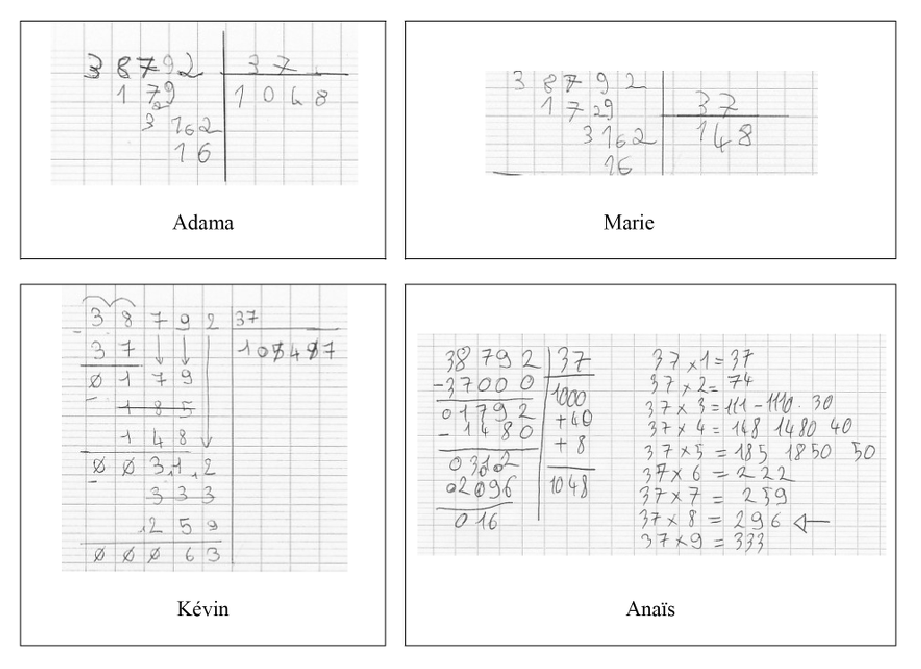
\includegraphics[width=15cm]{Nombres_et_calculs_did/Images/Num3_analyse_divisions}
\end{center}
\begin{enumerate}
   \item Donner un avantage de chacune des techniques opératoires utilisées par Adama et Anaïs.
   \item Relever les erreurs faites par Marie et Kévin et, pour chacune, émettre une hypothèse sur son origine.
\end{enumerate}
\end{exercice}

%\begin{center}
%   {\bf\large CRPE 2008 G6 : page 88 du manuel Euromaths} \\ [5mm]
%   \includegraphics[width=15cm]{Nombres_et_calculs_did/Images/Num8_2008_G6}
%\end{center}

\begin{corrige}
\ \\ [-5mm]
\begin{enumerate}
   \item Pour {\bf Adama}, il s'agit de la division euclidienne usuelle sans pose des soustractions intermédiaires. \\
   Un avantage est un gain de temps si l'élève est expert en calcul mental ainsi qu'un gain de place. \\
   Un inconvénient est sa complexité : il faut effectuer divers calculs mentalement, elle est donc source d'erreurs et de surcharge cognitive. \\ 
   Pour {\bf Anaïs}, il s'agit d'une procédure avec écriture de la table de multiplication du diviseur et de résultats intermédiaires reprenant à chaque étape la totalité du dividende. \\
   Quelques avantages : elle donne du sens à l'opération et elle évite la surcharge cognitive en ayant écrit les multiples de 37. De plus, un quotient non optimal lors d'une étape peut être rattrapé lors des étapes suivantes. \\
   Un inconvénient est la lourdeur de l'écriture.
   \item {\bf Marie} se trompe au niveau du quotient : elle oublie de mettre un \og zéro \fg{} entre le 1 et le 4. Cette erreur vient probablement du fait que dans 17, elle ne peut pas mettre 37, elle abaisse alors le chiffre suivant, sans penser à caractériser cette impossibilité par un 0 qui correspond au nombre de centaines du quotient. \\   
   {\bf Kévin} pose son opération en effectuant les soustractions intermédiaires. Il ne calcule pas à l'avance les multiplications et lorsqu'il se trompe, il barre sa réponse et reprend ensuite jusqu'à trouver une solution convenable. Lors de sa dernière étape, le calcul de $9\times37$ donne un résultat trop grand pour être soustrait, il tente donc la multiplication par 7 ce qui fonctionne. Cependant, il ne s'est pas aperçu que le reste obtenu est  supérieur au diviseur. La longueur de l'opération est peut-être en cause, et le calcul du répertoire multiplicatif de 37 aurait pu l'aider à calculer cette division de manière moins aléatoire.
\end{enumerate}
\end{corrige}

\bigskip

%%%%%%%%%%%%%%%%
%\begin{exercice*}[CRPE 2015 G3]
%L'exercice ci-dessous a été donné en évaluation à des élèves de CM1.
%\begin{center}
%\fbox{\begin{minipage}{12cm}
%   {\it Une école organise une sortie de fin d'année. \\
%   Pour se déplacer, le directeur loue des bus qui peuvent accueillir 42 passagers chacun. \\
%   Il y a 157 élèves dans l'école et 20 adultes les accompagneront. \\
%   Combien faut-il réserver de bus ?}
%\end{minipage}}
%\end{center}
%\begin{enumerate}
%   \item Quelle opération mathématique est l'enjeu de ce problème ?
%   \item Ci-dessous, sont présentées les productions de trois élèves A, B et D. Pour chacune d'elles, expliquer la procédure utilisée.
%   \item Un autre élève de la classe a effectué la division de 157 par 20. À quelle question ce calcul pourrait-il répondre ?
%   \item La situation du problème de départ et celle de la question 3) illustrent deux sens
%différents de la division. Les expliciter.
%\end{enumerate}
%
%\begin{center}
%   \fbox{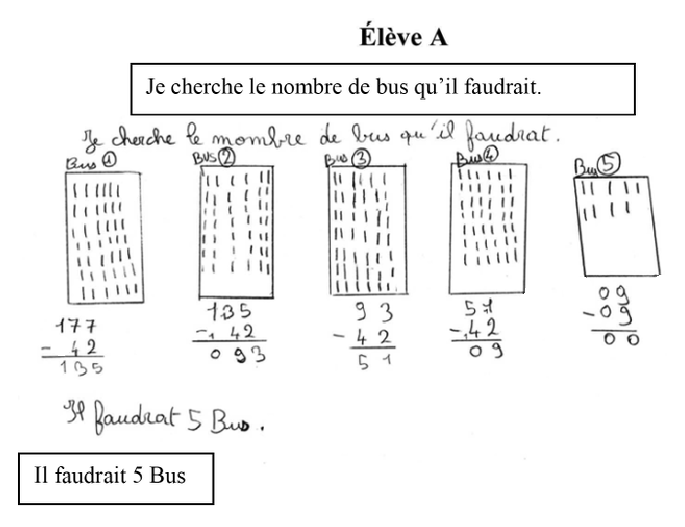
\includegraphics[width=11cm]{Nombres_et_calculs_did/Images/Num3_analyse_eleveA}} \\ [2mm]
%   \hspace*{-1cm}\fbox{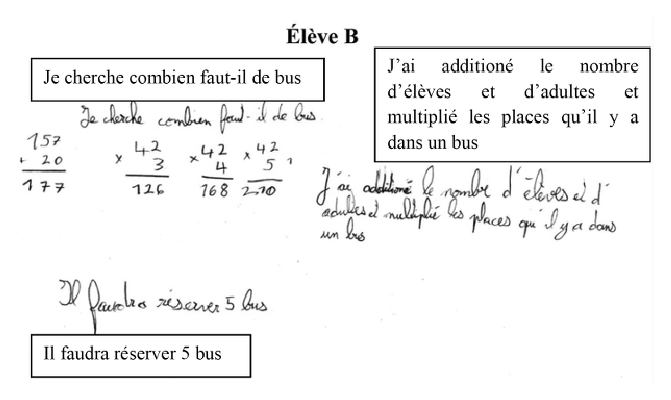
\includegraphics[height=5.5cm]{Nombres_et_calculs_did/Images/Num3_analyse_eleveB}}
%   \fbox{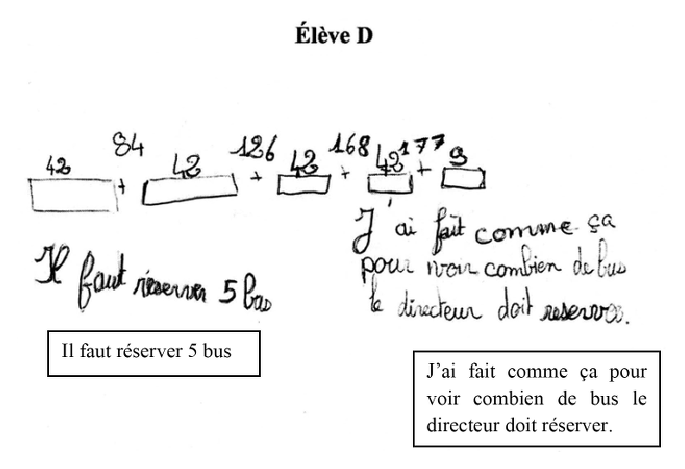
\includegraphics[height=5.5cm]{Nombres_et_calculs_did/Images/Num3_analyse_eleveD}}\hspace*{-1cm}
%\end{center}
%\end{exercice*}
%
%\begin{corrige}
%\ \\ [-5mm]
%\begin{enumerate}
%   \item L'opération en jeu de ce problème est la division euclidienne.
%   \item {\bf L'élève A} procède par schématisation : il représente les bus par des rectangles dans lesquels il dessine 42 traits représentent les passagers, un par un. Après avoir complété un bus, il calcule par une soustraction le nombre de passagers qu'il reste à placer. Il procède ainsi jusqu'à ce qu'il n'y ait plus aucun passager. Il conclut correctement. \\ 
%{\bf L'élève B} commence par déterminer le nombre total de passagers en posant l'addition. Puis, il effectue des multiplications de 42 par 3, puis 4 et 5. Il constate que 4 bus ne suffisent pas et que 5 bus conviennent. Il conclut correctement. \\ 
%{\bf L'élève D} schématise les bus par des rectangles contenant 42 personnes et effectue les additions itérées de 42 entre chaque paire du bus. Quand il parvient à 168, qui est proche du résultat, il détermine le nombre de personnes présentes dans le dernier bus et conclut correctement.
%   \item Il y a 157 élèves et 20 adultes. On souhaite faire des groupes équitable d'élèves pour chaque adulte. Combien d'élèves y a-t-il dans chaque groupe ?
%   \item Pour la situation du problème de départ, il s'agit de la division quotition qui répond à la question : \og Combien de paquets de 42 unités peut on faire avec 177 unités ? \fg. \\
%Pour la situation de la question 3), il s'agit de la division partition qui répond à la question : \og On dispose de 20 paquets. Combien d'unités comprendra chaque paquet sachant qu'il y a au total 177 unités et que chaque paquet dispose du même nombre d'unités ? \fg. \\
%Dans les deux cas, il faudra prendre en compte le fait que le reste de la division euclidienne n'est pas nul.
%\end{enumerate}
%\end{corrige}
%
%\bigskip

\bigskip


\begin{exercice}[CRPE 2017 G2]
Exercice extrait des évaluations nationales à l’entrée au CE2.
\begin{center}
\fbox{
\begin{minipage}{12cm}
   Un fermier range 6 oeufs dans chaque boîte. \\
   Quand il a fini, il compte ses boîtes et en trouve 13. Combien a-t-il rangé d'oeufs ? \\
   Écris tes calculs dans le premier cadre et ta réponse dans le deuxième cadre.
\end{minipage}
}
\end{center}
On a ci-dessous les productions de six élèves.
\begin{enumerate}
   \item Pour chacun des élèves 1, 2 et 3 : expliciter les procédures utilisées et donner deux compétences qui semblent acquises par chacun des élèves.
   \item Pour chacun des élèves 4, 5 et 6 : citer une compétence qui semble acquise, identifier et analyser les erreurs.
   \item Pour l’élève 5, proposer une aide que pourrait envisager l’enseignant pour l’amener à corriger son erreur.
   \item Pour les élèves 1 et 6, comment l’enseignant pourrait-il modifier l’énoncé pour les amener à utiliser une multiplication ?
\end{enumerate}
\vspace*{-0.4cm}
\begin{center}
   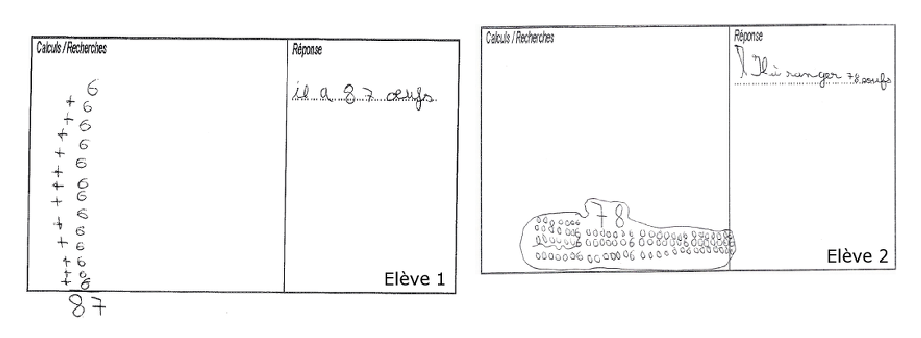
\includegraphics[width=15.2cm]{Nombres_et_calculs_did/Images/Num3_analyse_E12} \\
   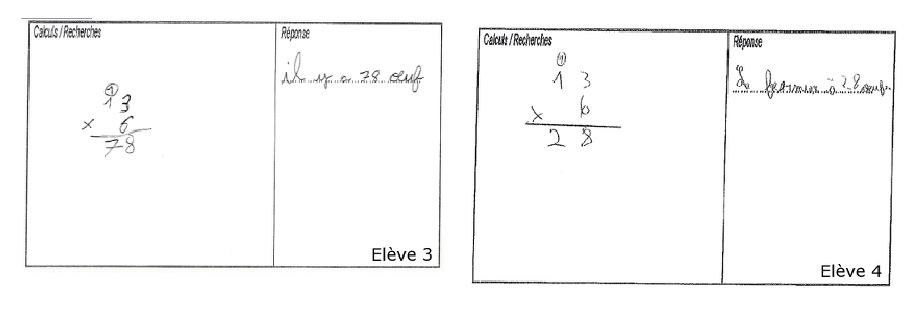
\includegraphics[width=15.2cm]{Nombres_et_calculs_did/Images/Num3_analyse_E34} \\
   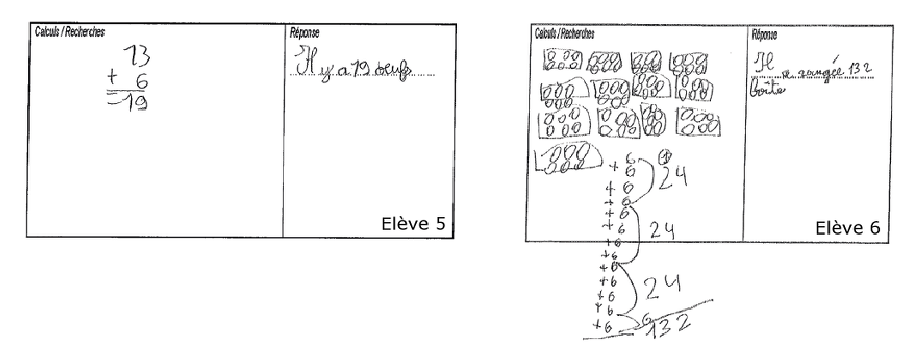
\includegraphics[width=15.2cm]{Nombres_et_calculs_did/Images/Num3_analyse_E56}
\end{center}
\vspace*{-1cm}
\end{exercice}

\begin{corrige}
\ \\ [-5mm]
\begin{enumerate}
   \item {\bf Élève 1 : } il effectue une addition itérée de 6 (\oe ufs), treize fois, qu'il pose en colonne. Le résultat est 78, on ne sait pas si l'élève s'est trompé dans son opération ou s'il s'est trompé en notant le résultat (échange de la dizaine et de l'unité). \\
   L'élève 1 sait résoudre un problème dans le champ additif, et il sait modéliser correctement la situation par une opération mathématique correcte : l'addition itérée. \\
   {\bf Élève 2 : } il modélise la situation par un schéma dans lequel il dessine des paquets de 6 \oe ufs en prenant soin d'indiquer le nombre d'\oe ufs à côté de chaque paquet. Puis il compte les \oe ufs un à un, ou six par six jusqu'à obtenir 78, qui est un résultat juste. \\
   L'élève 2 sait résoudre un problème dans le champ additif, il sait modéliser correctement la situation par un schéma et utiliser ce schéma pour dénombrer. \\
   {\bf Élève 3 : } il effectue la multiplication de 13 (boites) par 6 (\oe ufs) et obtient un résultat juste. Il s'agit ici de la procédure experte. \\
   L'élève 3 sait résoudre un problème dans le champ multiplicatif, il sait modéliser correctement la situation et maitrise la technique opératoire de la multiplication posée en colonne. \\
   \item {\bf Élève 4 : } il effectue la multiplication de 13 (boites) par 6 (\oe ufs), il sait donc résoudre un problème dans le champ multiplicatif en posant la bonne opération experte. \\
   Le résultat de $3\times6$ est juste : 18, il pose bien ses deux chiffres dans l'opération mais ensuite semble effectuer la somme de 1 et de 1, ceci est probablement dû au fait que les deux nombres n'ont pas le même nombre de chiffres, et après avoir utilisé une fois le \og 6 \fg{}, il additionne la retenue à la dizaine comme il le ferait dans une addition. \\
   {\bf Élève 5 : } il sait effectuer une addition posée en colonnes. \\
   Par contre, il ne sait pas modéliser la situation par la bonne opération. \\
   {\bf Élève 6 : } il sait schématiser la situation et poser le calcul adéquat. \\
   Il regroupe les \og 6 \fg{} par paquets de 4 pour obtenir 24, qu'il indique à côté de chaque paquet, ce qui est juste. Enfin, il effectue l'opération $24+24+6$ en colonnes, mais son \og 6 \fg{} n'est pas bien placé et il le calcule comme étant un chiffre de la colonne des dizaines, son résultat final est donc faux.
   \item Pour l’élève 5, on peut lui proposer de schématiser la situation, et de commencer à dénombrer les \oe ufs, il se rendrait vite compte que 19 est trop petit. Ensuite, on pourrait lui proposer d'écrie le calcul de plusieurs façons différentes (somme, produit) afin de lui faire découvrir quelle procédure est la plus rapide.
   \item Pour les élèves 1 et 6, il suffirait de donner un nombre de boites bien plus élevé (par exemple, 67), pour que la procédure par schématisation soit longue et fastidieuse et que les élèves soient contraints à réfléchir à une autre méthode, plus rapide.
\end{enumerate}
\end{corrige}

\bigskip


%\begin{exercice}[CRPE 2018 G3]
%Voici une situation problème proposée à des élèves de CM1 et trois productions illustrant sa résolution :
%\begin{center}
%\fbox{
%\begin{minipage}{12cm}
%   Combien de sacs de 12 billes peut-on faire avec 56 billes ?
%\end{minipage}
%}
%\end{center}
%\begin{center}
%   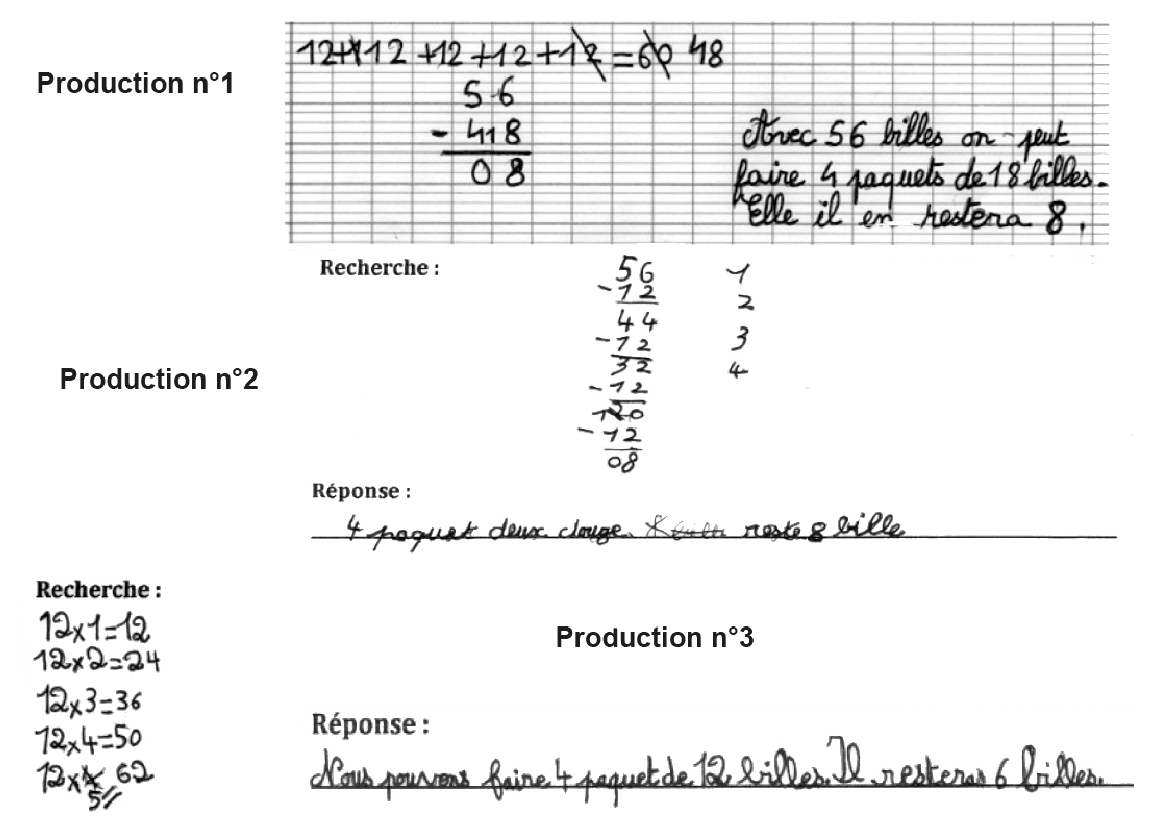
\includegraphics[width=14.5cm]{Nombres_et_calculs_did/Images/Num3_analyse_billes}
%\end{center}
%\begin{enumerate}
%   \item Pour chacune de ces productions, expliciter la procédure utilisée pour résoudre le problème.
%   \item Expliquer comment la modification des nombres de l’énoncé peut montrer les limites des procédures mises en oeuvre et inciter à l’utilisation de la technique opératoire de la division ?
%   \item Citer trois connaissances ou capacités nécessaires pour effectuer une division posée ?
%\end{enumerate}
%\end{exercice}
%
%\begin{corrige}
%\ \\ [-5mm]
%\begin{enumerate}
%   \item Procédure utilisées pour résoudre le problème.
%   \begin{itemize}
%      \item {\bf Production n\degres1} : procédure progressive dans le champ additif (additions). \\
%      L'élève additionne le nombre 12 cinq fois à la suite, il trouve 60. Ce nombre étant supérieur à 56, il barre un \og 12 \fg{} et recalcule la somme qui vaut 48. Ce nombre est inférieur à 56. Ensuite, il effectue la soustraction de 48 à 56 pour trouver ke nombre de billes restantes. Il lui reste à compter le nombre de \og 12 \fg{} additionnés pour conclure qu'il peut faire 4 paquets de 12 billes et qu'il en reste 8.
%      \item {\bf Production n\degres2} : procédure progressive dans le champ additif (soustractions). \\
%      L'élève soustrait 12 à 56 pour trouver 44, puis il réitère ce procédé jusqu'à trouver un nombre inférieur à 12 (on note que, même si la procédure est correcte, l'écriture mathématique en colonnes n'est pas valable à partir du deuxième calcul). Il note à côté chaque paquet de 12 qu'il soustrait, il en trouve 4 et il reste 8 billes.
%      \item {\bf Production n\degres3} : procédure progressive dans le champ multiplicatif (multiplications). \\
%      Cet élève calcule le répertoire multiplicatif de 12 jusqu'à obtenir un encadrement de 56, il semble effectuer les calculs en additionnant à chaque fois 12, étant donné son erreur à $12\times4$ (il a un écart de 2 avec le résultat réel, cet écart est répercuté sur le dernier calcul). Sa réponse est cohérente.
%   \end{itemize}
%   \item Les procédures mises en \oe uvre sont acceptable puisqu'elles ne demandent pas trop de calculs : tous les élèves effectuent des calculs de proche en proche qui aboutissent assez rapidement au résultat. Cependant, si on choisissait un nombre bien plus grand (par exemple 1\,246), les calculs seront trop longs et fastidieux et les élèves devraient penser à une autre procédure. On peut également faire varier le nombre de billes dans chaque sac (par exemple 57) pour que les calculs soient moins évident à calculer mentalement. \\
%   Cette situation est donc intéressante dans un premier temps et doit évoluer par la suite avec des nombres plus grands afin de transiter petit à petit vers la méthode experte qui consiste à effectuer une division euclidienne pour une division-quotition.
%   \item On peut citer les connaissances ou capacités suivantes :
%   \begin{itemize}
%      \item connaissance : connaître ses tables de multiplication et d'addition ;
%      \item capacité : effectuer une multiplication, une soustraction (pour les calculs intermédiaires) ;
%      \item capacité : savoir faire une approximation afin de trouver  le nombre de chiffres au quotient ainsi que le meilleur nombre au quotient par exemple par essai-erreur.
%   \end{itemize}
%\end{enumerate}
%\end{corrige}


\newpage


\begin{exercice}[CRPE 2017 G3]
On considère l’exercice suivant issu du manuel scolaire \og Cap maths \fg, Hatier (édition 2016).
\begin{center}
   \fbox{
   \begin{minipage}{7cm}
      {\bf Calcule avec la méthode de ton choix.} \\
      a. $91-52 =$ \dots{} \dots \hfill  c. $800-153=$ \dots{} \dots \\
      b. $613-209 =$ \dots{} \dots  \hfill d. $607-54=$ \dots{} \dots
   \end{minipage}}
\end{center}
\begin{enumerate}
   \item Quelle est la notion abordée ? Citer deux connaissances et savoir-faire que cette situation met en jeu.
   \item Étude des productions des élèves. On considère les quatre productions d’élèves ci-dessous.
   \begin{enumerate}
      \item Quelles sont les différentes procédures utilisées par Antoine, Barbara et Clara ?
      \item Qu’est-ce qui différencie les procédures utilisées par Barbara et Dominique ?
      \item Relever les réussites et les erreurs de Barbara et Clara.
      \item Quel accompagnement pédagogique mettre en \oe uvre pour remédier aux difficultés rencontrées par Clara ?  \\ [-8mm]
   \end{enumerate}
\end{enumerate}
\begin{center}
   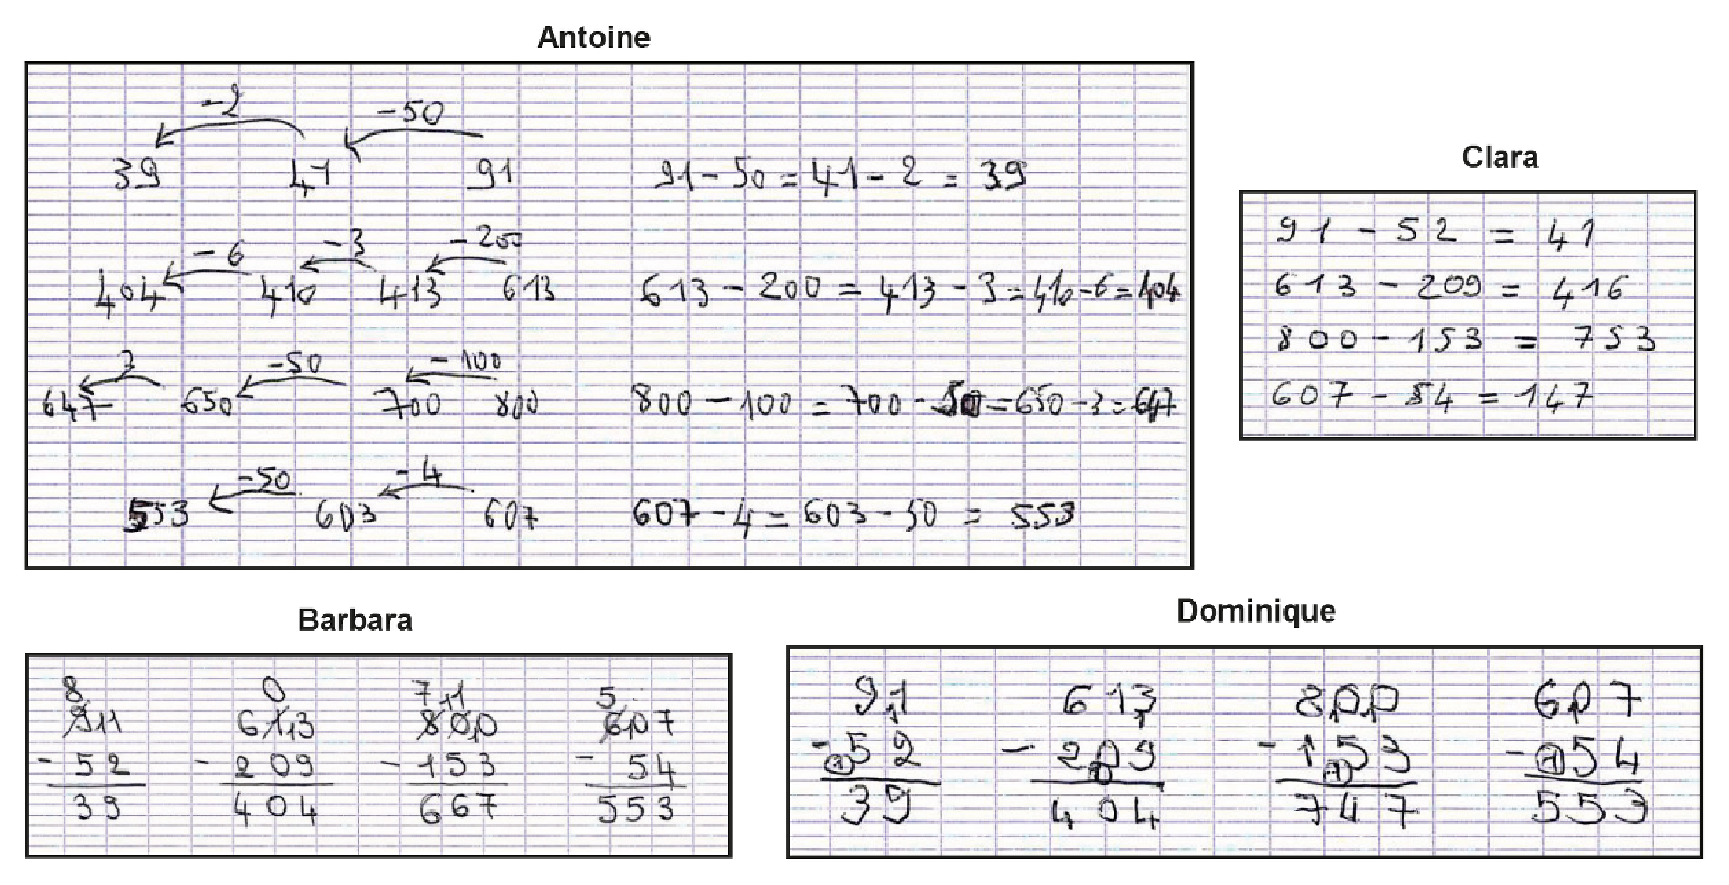
\includegraphics[width=14.5cm]{Nombres_et_calculs_did/Images/Num3_analyse_soustractions}
\end{center}
\end{exercice}

\begin{corrige}
\ \\ [-5mm]
\begin{enumerate}
   \item La notion abordée est la soustraction, l'élève doit effectuer une soustraction par la méthode de son choix (développer l'algorithme) : par un calcul en ligne ou par un calcul en colonnes (soustraction classique, par emprunts ou comme addition à trous), et doit avoir des connaissances en calcul mental (répertoire additif).
   \item
      \begin{enumerate}
         \item {\bf Antoine} utilise une procédure de calcul en ligne par soustractions successives. Il part du nombre le plus grand et décompose le nombre à retirer : il commence par enlever le plus grand multiple de 100 s'il existe, puis le plus grand multiple de 10 et enfin les unités, sauf pour le dernier calcul. Ensuite, il écrit le calcul en ligne, les résultats sont justes mais mal écrits d'un point de vu mathématique (statut du signe \og = \fg).\\
         {\bf Barbara} effectue des soustractions posées en colonnes grâce à la méthode par emprunts. \\
         {\bf Clara} effectue des calculs en ligne, elle soustrait pour chaque rang le plus petit nombre au plus grand, en commençant par le chiffre le plus à gauche (on le devine grâce à la dernière opération).
      \end{enumerate}
\end{enumerate}

\Coupe

\begin{enumerate}
   \begin{enumerate}
      \setcounter{enumii}{1}
      \item {\bf Barbara} utilise la méthode par emprunts : si besoin, elle emprunte une unité au rang supérieur, qu'elle donne au rang actuel en cassant cette unité en dix. \\
      {\bf Dominique} effectue des soustractions par la méthode classique basée sur le principe des différences constantes : lorsque la valeur du chiffre du haut est inférieure à celle du chiffre du bas, il ajoute 10 unités du rang en haut et une unité du rang supérieur en bas.
      \item {\bf Barbara} effectue correctement les opérations a., b. et d. Par contre, elle se trompe dans l'opération c., erreur classique de la méthode lorsque le nombre le plus grand comporte un ou plusieurs \og 0 \fg. Elle a besoin d'emprunter une dizaine, mais 800 ne comporte pas de chiffre des dizaines, il faut donc emprunter une centaine, il en reste bien 7 et on a 10 dizaines. Elle semble ensuite reporter un \og 1 \fg{} au lieu d'ôter la dizaine du départ. Elle effectue donc $11-5$ au lieu de $9-5$. \\
      {\bf Clara} n'a aucun résultat de juste car sa procédure n'a aucun sens.
      \item Pour Clara, il faut revoir la soustraction posée au niveau de son sens. Pour cela, on peut revenir aux bases et conceptualiser la soustraction grâce à un matériel pédagogique (pièces et billets par exemple). \medskip
   \end{enumerate}
\end{enumerate}
\end{corrige}



\begin{exercice}[CRPE 2017 G1]
   L'exercice ci-dessous est extrait de évaluations nationales CM2 de 2012.
   \begin{center}
   \fbox{
      \begin{minipage}{12cm}
         Il faut 9 litres d’huile pour remplir complètement 5 bidons identiques. \\
      Quelle est la contenance, en litre, de chacun de ces bidons ?
      \end{minipage}
   }
   \end{center}
   \begin{enumerate}
      \item Quelle opération permet de répondre à cette question ?
      \item Voici les productions de Julia, Karima et Louis. Pour chacune d’entre elles, expliquer la procédure utilisée.
      \item Quelles modifications, concernant les nombres en jeu dans l’exercice, peut proposer l’enseignant à Louis pour l’encourager à changer de procédure ? \vspace*{-0.4cm}
   \end{enumerate}
   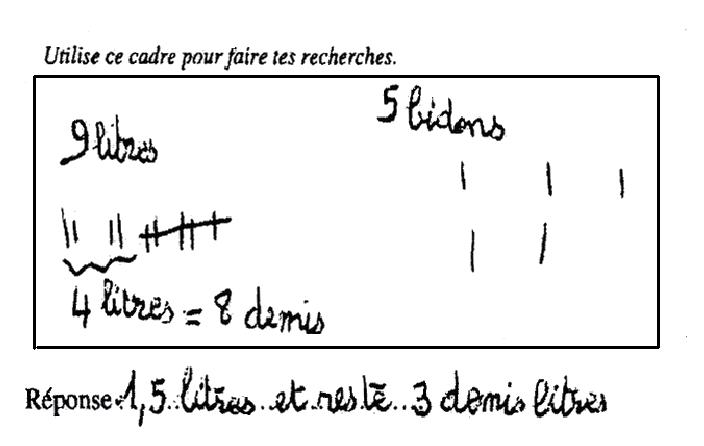
\includegraphics[height=3.2cm]{Nombres_et_calculs_did/Images/Num3_analyse_Julia} 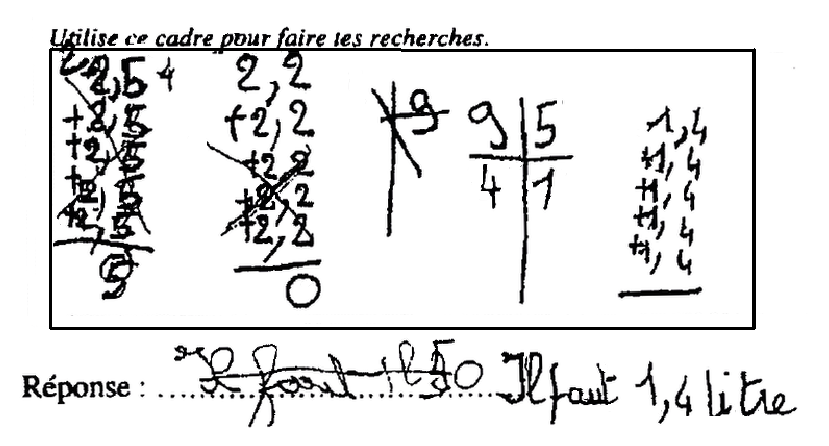
\includegraphics[height=3.2cm]{Nombres_et_calculs_did/Images/Num3_analyse_Karima}  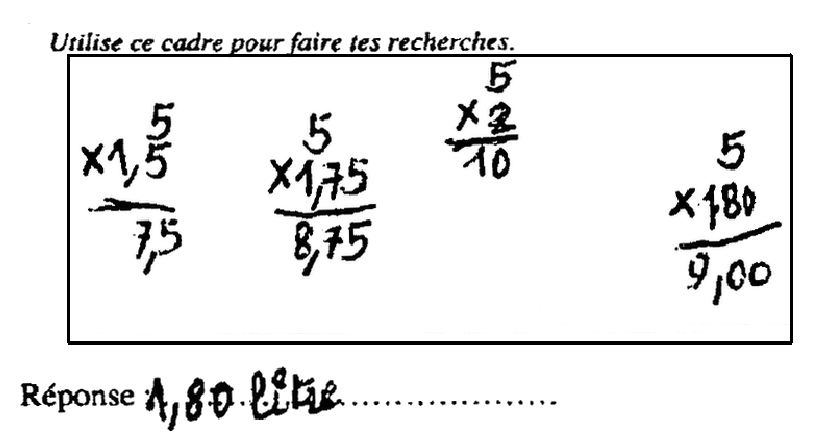
\includegraphics[height=3.2cm]{Nombres_et_calculs_did/Images/Num3_analyse_Louis}
\end{exercice}

\begin{corrige}
\ \\ [-5mm]
\begin{enumerate}
   \item Une \textbf{division décimale} permet de répondre à la question, et plus particulièrement la division de deux nombres entiers avec quotient décimal : $\opdiv[decimalsepsymbol={,}]{9}{5}$. \quad La réponse attendue est donc 1,8 L. \\
   \item \textbf{Julia} schématise la situation par 9 bâtons pour les 9 litres d'huile et 5 bâtons pour les 5 bidons. Ensuite, elle associe 5 litres à 5 bidons en barrant 5 bâtons. Il lui reste 4 litres qu'elle transforme en 8 demi-litres. Parmi ces 8 demi-litres, elle en attribue 5 aux 5 bidons ce qui lui donne un litre plus un demi-litre, soit 1,5 litre par bidon. Il lui reste 3 demi-litres qu'elle laisse ainsi. \\
      Son raisonnement n'est pas faux, son résultat est cohérent mais il ne correspond pas tout à fait à la question. \\
   \textbf{Karima} commence par procéder par essais-erreurs : elle fait une addition itérée de 2,5 (5 fois), elle calcule la somme des dixièmes et il semble qu'elle calcule également la somme des unités mais qu'elle ne l'écrive pas car la valeur n'est pas celle qu'elle doit trouver. Elle se rend compte néanmoins que le résultat est trop grand, et c'est la raison pour laquelle elle teste la même procédure avec 2,2. \\
      Après deux tentatives, elle cherche une autre procédure plus efficace, elle pense à une division en commençant par une division par 9, qu'elle barre rapidement pour effectuer la division de 9 par 5, ce qui est une procédure experte. Cependant, elle fait une division euclidienne qui ne donne pas un résultat, mais deux (quotient et reste) qui ne lui permettent théoriquement pas de conclure. Elle répond en donnant un résultat composé du quotient comme chiffre des unités, et du reste comme chiffre des dixième, ce qui démontre une mauvaise compréhension des termes obtenus dans une division euclidienne et de la maîtrise des nombres décimaux. Enfin, elle tente une vérification avec le nombre 1,4 trouvé, mais elle n'effectue pas le calcul. \\
      Son résultat est erroné.
   \textbf{Louis} procède par essais-erreurs également mais avec une procédure plus rapide : il cherche la valeur en effectuant la multiplication. Il commence par multiplier par 5 par 1,5, son résultat est trop petit. Il tente donc 1,75, c'est toujours trop petit. Puis il essaie avec 2, le résultat est trop grand, enfin il tente avec 1,8 ce qui lui donne le bon résultat. \\
      Sa réponse est correcte. 
   \item Si l'objectif est d'utiliser la technique experte (la division décimale), le quotient ne peut être qu'un nombre entier, donc le nombre de bidons est un nombre entier. \\
   En revanche, on peut \textbf{modifier le nombre de litres} de manière à rendre la procédure par essais-erreurs plus longue, par exemple en choisissant 9,1 litres.
\end{enumerate}
\end{corrige}


%%%%%%%%%%%%%
\Recreation %%%%%%%
%%%%%%%%%%%%%

\setcounter{exercice}{0}
\begin{exercice*}[\fbox{C1} - Fabriquer un album à compter] %%% 
   \begin{description}
      \item[Compétence visée] : travailler les différentes désignations des nombres.
      \item[Objectif] : donner du sens aux nombres en les matérialisant de différentes façons. Les diverses désignations du nombre (chiffres, mots, représentations digitales, dés, collections d'objets, jetons\dots) contribuent à structurer les connaissances. Le champ numérique utilisé est choisi en fonction des compétences des élèves. 
      \item[Déroulement] : 
      \begin{enumerate}
         \item Découvrir des livres à compter. \\
           Par exemple : \href{https://www.youtube.com/watch?v=6uPh8zpPias}{\it\blue 1, 2, 3 petits chats qui savent compter jusqu'à 3} ; \href{https://www.youtube.com/watch?v=lQOk4qjXq0E}{\it\blue Cinq petites coccinelles} ; \href{https://www.glenat.com/histoires-pour-compter/dix-petites-coccinelles-9782841961924}{\it\blue 10 petites coccinelles}\dots
         \item Organiser le projet :
         \begin{itemize}
            \item combien de pages ?
            \item quels éléments : écriture chiffrée, écriture en lettres, représentation digitale, constellation du dé, collection d'objet, frise, abaque\dots ?
            \item quelles techniques : dessiner, colorier, peindre, coller, utiliser des tampons\dots ?
            \item quel format : une double page par nombre ou pages découpées à reconstituer ?
         \end{itemize}
         \item Accompagner le projet : apprendre des comptines, travailler sur les collections (classer, catégoriser, comparer), ritualiser des jeux mathématiques ;
         \item Concevoir et fabriquer : peut se faire tout au long de l'année, en fil rouge ;
         \item Faire partager : présenter le livre à une autre classe, ramener son livre à la maison.
      \end{enumerate}
      \item[Exemples] : \href{http://maternelle27.spip.ac-rouen.fr/IMG/pdf/8._les_livres_acompter.pdf}{\it\blue Projet : réalisation d'un livre à compter}
   \end{description}
\end{exercice*}

\begin{center}
   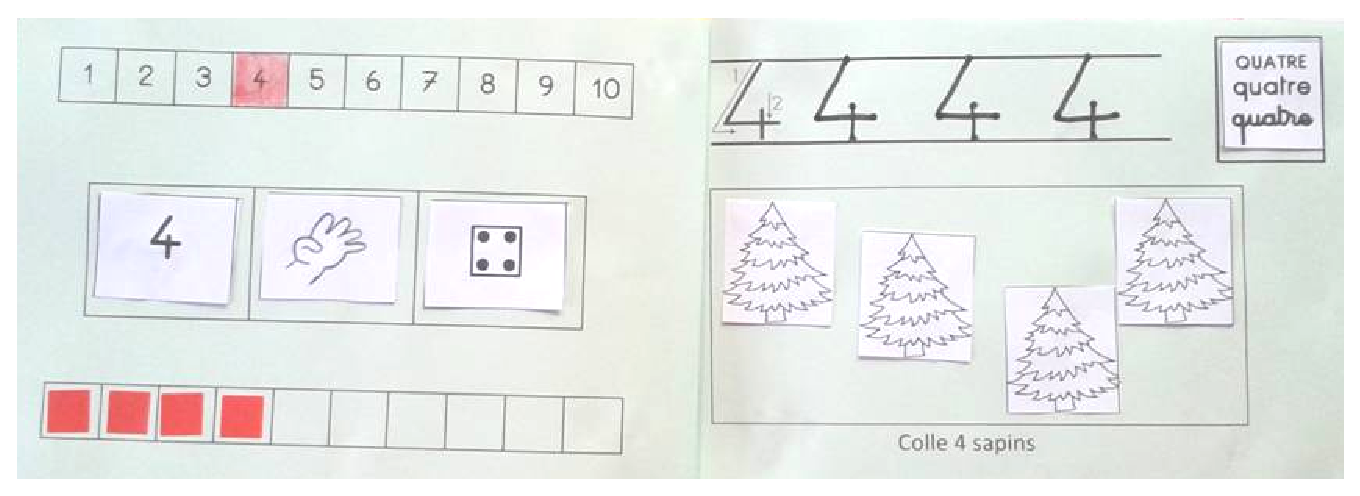
\includegraphics[width=15cm]{Nombres_et_calculs_did/Images/Num3_activites_page_album} \\
   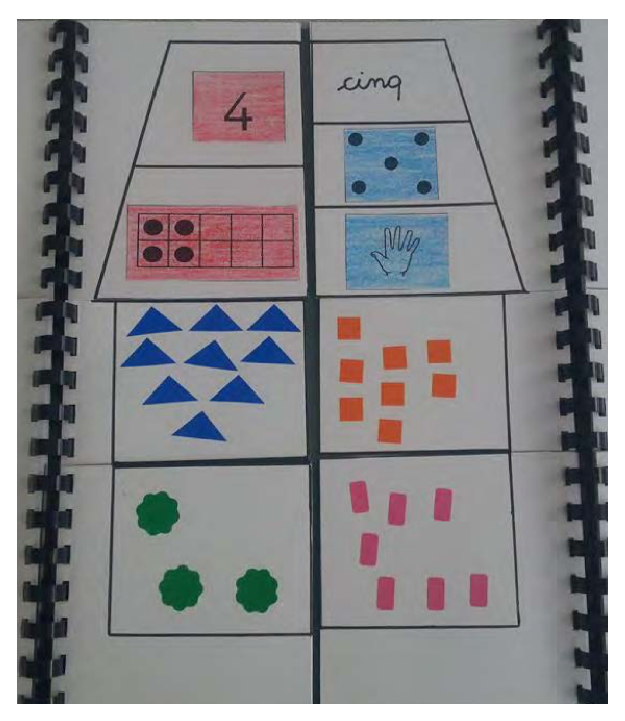
\includegraphics[width=6cm]{Nombres_et_calculs_did/Images/Num3_activites_album_calcul}
\end{center}


\bigskip

\begin{exercice*}[\fbox{C1} - Greli-grelo] %%% 2 %%%
   \begin{description}
      \item[Compétence visée] : composer, décomposer les nombres.
      \item[Objectif] : déterminer le nombre d'objets d'une collection après augmentation ou diminution de ce nombre sans que la collection entière soit visible.
      \item[Déroulement] : le meneur de jeu place des objets dans une main, il montre cette main ouverte pour que les élèves puissent dénombrer les objets qu'il place dans une boîte opaque.
Il fait ensuite de même avec son autre droite et place les objets contenus dans cette main dans la même boîte. Il ferme la boîte et la secoue en chantant : \og Greli-grelo, combien j'ai d'sous dans mon sabot ? \fg. On écoute les propositions des autres joueurs et on valide en recomptant la totalité des objets sortis de la boîte et étalés sur un plateau. 
      \item[Variantes] : types de jetons, nombre de jetons, cartes de constellations, retirer des jetons, commence par montrer la collection complète puis une partie de la collection\dots
      \item[Exemples] : \href{https://www.youtube.com/watch?v=nM750kaM6zo}{\it\blue Greli-grelo décomposition}, \href{https://www.youtube.com/watch?v=qj_1ht_FXsg}{\it\blue Greli-grelo  composition}. \\
   \end{description}
\end{exercice*}

\bigskip


\begin{exercice*}[\fbox{C1} - Halli Galli]
   \smallskip
   
   {\it Source : Vers les maths, moyenne section. Accès.} \smallskip
   
   {\bf Matériel} : 56 cartes où sont dessinés de 1 à 5 fruits (banane, pruneau, fraise, citron), une sonnette, des jetons. \smallskip

   {\bf Organisation :} travail dirigé avec 4 élèves. \smallskip

   {\bf Déroulement}
   \begin{description}
      \item[Étape 1 :] Découvrir les cartes de Halli Galli
         \begin{itemize}
            \item Observer les cartes. Nommer les fruits. Dire combien de fruits l’on voit. \\
               Trier les cartes en fonction du nombre de fruits.
            \item Trier les cartes en fonction du type de fruit. Se répartir la tâche dans le groupe. Chaque élève classe ensuite ses cartes en fonction du nombre de fruits. Ranger les paquets de cartes dans l’ordre croissant
         \end{itemize}
   
      \item[Étape 2 :] Retrouver tes décompositions du nombre 5
         \begin{itemize}
            \item Étaler toutes les cartes fraises et bananes sur la table faces fruits visibles. \\
               Prendre deux cartes chacun son tour pour faire 5. Les cartes doivent représenter la même sorte de fruit. \\
               Si l’élève réussit, il reçoit un jeton. Dans le cas contraire, il repose les cartes et passe son tour.
            \item Mettre en commun les moyens pour savoir si les deux cartes font 5 : dénombrer les fruits en utilisant la suite orale des nombres, surcompter en utilisant la suite orale des nombres.
         \end{itemize}

      \item[Étape 3 :] Jouer à Halli Galli  
         \begin{itemize}
            \item {\it Jeu 1 : Découvrir la sonnette} \\
               L’enseignant forme un tas devant lui avec les cartes de 5 fruits et quelques autres. \\
               La clochette est posée au centre de la table à la même distance de chaque joueur.
               \begin{itemize}
                  \item[--] L’enseignant retourne une carte. Si cette carte représente 5 fruits, le joueur qui sonne le premier gagne la carte. On joue seulement quelques minutes à ce jeu pour que chaque élève utilise la sonnette au moins une fois. 
               \end{itemize}

      \item {\it Jeu 2 : Jouer avec deux cartes} \\
         L’enseignant pose deux tas de cartes devant lui. Il n’utilise que les cartes bananes et fraises.
         \begin{itemize}
            \item[--] L’enseignant retourne deux cartes. Si 5 fruits de la même sorte figurent parmi les cartes retournées, le joueur qui sonne le premier gagne les deux cartes. 
         \end{itemize}
         
      \item {\it Jeu 3 : Jouer selon la règle de Halli Galli}
         \begin{itemize}
            \item[--] Les cartes sont distribuées une à une à chaque joueur jusqu’à ce qu’il n’en reste plus.
            \item[--] Chaque joueur pose son tas de cartes à l’envers devant lui.
            \item[--] Chaque joueur retourne à tour de rôle la première carte de son tas et la place devant lui.
            \item[--] Dès que 5 fruits de la même sorte figurent parmi les cartes retournées, le joueur qui sonne le premier gagne les deux cartes qui additionnées font 5. Il donne les cartes gagnées à l’enseignant et reçoit un jeton en échange.
            \item[--] Lorsque toutes les cartes ont été retournées et qu’il n’y a plus de possibilité de faire 5, on compte le nombre de jetons gagnés par chaque joueur.
            \item[--] Si un joueur sonne alors qu’il n’y a pas 5 fruits de la même sorte, il passe une fois son tour. \medskip
         \end{itemize}
      \end{itemize}
   \end{description}
   On trouvera sur le site \href{http://www.pedagogieautisme.fr/2018/02/jouer-a-halli-galli-activites-preparatoires-et-regle-du-jeu-modifiees.html}{\blue Maths - Jouer à Halli Galli} des variantes de ce jeu avec des fiches à imprimer.
   \begin{center}
      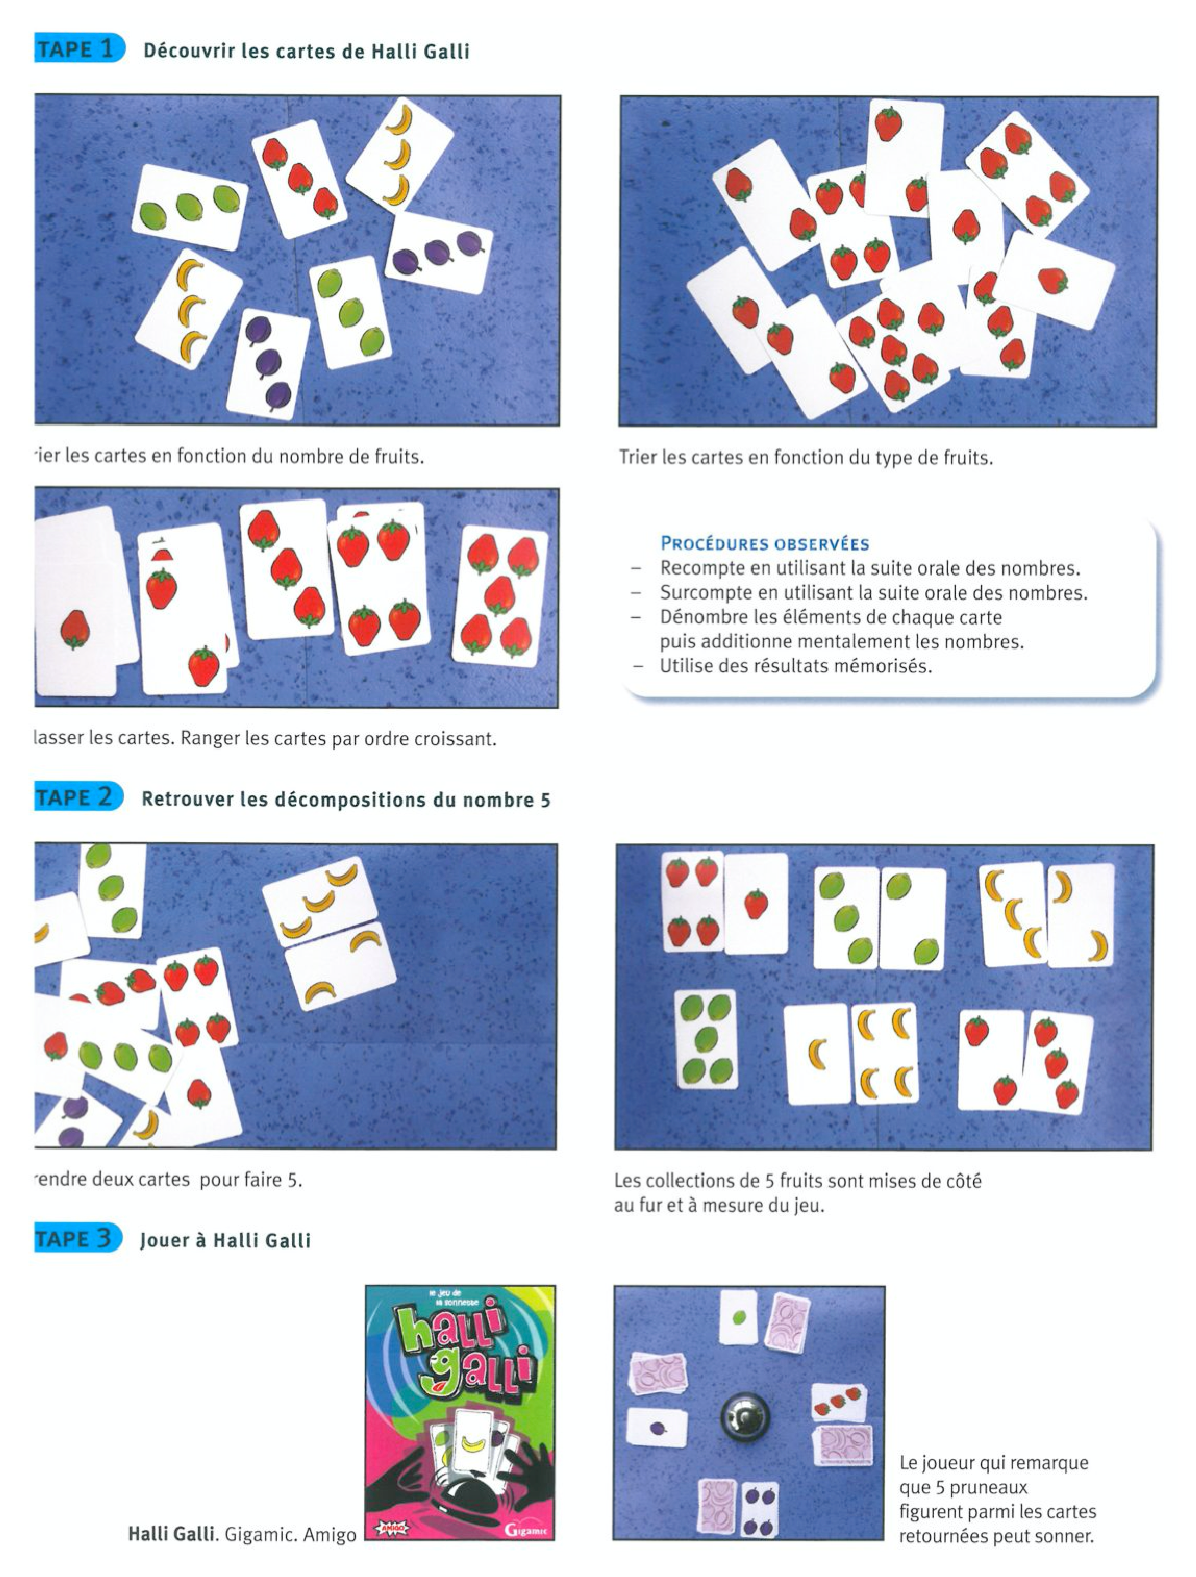
\includegraphics[width=12.5cm]{Nombres_et_calculs_did/Images/Num3_activites_Halli_galli}
   \end{center}
\end{exercice*}



\begin{exercice*}[\fbox{C2/C3} - La multiplication per gelosia]
      \partie[multiplication par un nombre à un chiffre]
         \parbox{7cm}{Leonardo a effectué la multiplication ci-contre. \\
            Faire l'opération à côté, comment Leonardo a-t-il fait son opération ?}
            \begin{pspicture}(-2,1)(4.5,2.5)
               \multido{\n=0+1}{4}{\psline(\n,1)(\n,2)}
               \multido{\n=1+1}{2}{\psline(0,\n)(3,\n)}
               \rput(0.5,2.3){1}
               \rput(1.5,2.3){2}
               \rput(2.5,2.3){3}
               \rput(3.25,1.5){3}
               \psline(1,2)(-0.5,0.5)
               \psline(2,2)(0.5,0.5)
               \psline(3,2)(1.5,0.5)
               \rput(2.3,1.7){\blue 0}
               \rput(2.7,1.3){\red 9} 
               \rput(1.3,1.7){\blue 0}
               \rput(1.7,1.3){\red 6} 
               \rput(0.3,1.7){\blue 0}
               \rput(0.7,1.3){\red 3}
               \rput(2.1,0.7){\bf 9} 
               \rput(1.1,0.7){\bf 6} 
               \rput(0.1,0.7){\bf 3} 
               \rput(1.5,0){$123\times3 =369$}
            \end{pspicture}
            
            \ \\ [5mm]
            \parbox{7cm}{Leonardo a ensuite effectué une multiplication plus difficile. \\
            Faire l'opération à côté, comment Leonardo a-t-il fait son opération ?}
            \begin{pspicture}(-2,1)(4.5,2.5)
               \multido{\n=0+1}{4}{\psline(\n,1)(\n,2)}
               \multido{\n=1+1}{2}{\psline(0,\n)(3,\n)}
               \rput(0.5,2.3){3}
               \rput(1.5,2.3){4}
               \rput(2.5,2.3){8}
               \rput(3.25,1.5){7}
               \psline(1,2)(-0.5,0.5)
               \psline(2,2)(0.5,0.5)
               \psline(3,2)(1.5,0.5)
               \rput(2.3,1.7){\blue 5}
               \rput(2.7,1.3){\red 6} 
               \rput(1.3,1.7){\blue 2}
               \rput(1.7,1.3){\red 8} 
               \rput(0.3,1.7){\blue 2}
               \rput(0.7,1.3){\red 1}
               \rput(2.1,0.7){\bf 6} 
               \rput(1.1,0.7){\bf 3} 
               \rput(0.1,0.7){\bf 4}
               \rput(-0.9,0.7){\bf 2}
               \rput(1.7,2.13){\tiny{$+1$}} 
               \rput(1.5,-0.2){$348\times7 =2\,436$}
            \end{pspicture}
            
            \ \\ [5mm]
            \parbox{7cm}{À la manière de Leonardo, effectue l'opération : $257\times6$.}
            \begin{pspicture}(-2,1)(4,2.5)
               \multido{\n=0+1}{4}{\psline(\n,1)(\n,2)}
               \multido{\n=1+1}{2}{\psline(0,\n)(3,\n)}
               \rput(0.5,2.3){2}
               \rput(1.5,2.3){5}
               \rput(2.5,2.3){7}
               \rput(3.25,1.5){6}
               \psline(1,2)(-0.5,0.5)
               \psline(2,2)(0.5,0.5)
               \psline(3,2)(1.5,0.5)
               \rput(1.5,-0.2){$257\times6 =\hdashrule{2cm}{0.15pt}{4pt 2pt}$}
            \end{pspicture}
 
   \ \\ [10mm]  
   Cette technique de multiplication s'appelle la {\bf multiplication per gelosia}, elle  vient de la civilisation indienne au {\small XII}\up{e} siècle, et a été introduite en Europe par le mathématicien italien {\bf Léonard de Pise}, plus connu sous le nom de {\bf Fibonacci}. Elle est très utilisée jusqu'au {\small XV}\up{e} siècle. \\
      Le nom fait allusion à la pièce en bois qui, en Italie, équipait certaines \og fenêtres à jalousie \fg{} chez les maris jaloux : la femme pouvait regarder ce qui se passait dans la rue sans être vue des autres hommes. 
      
Effectue les opérations suivantes en indiquant à côté l'opération réalisée et le résultat obtenu.
\\
      \begin{pspicture}(-3.5,0)(4,3)
      \multido{\n=0+1}{4}{\psline(\n,1)(\n,2)}
      \multido{\n=1+1}{2}{\psline(0,\n)(3,\n)}
      \rput(0.5,2.3){3}
      \rput(1.5,2.3){4}
      \rput(2.5,2.3){8}
      \rput(3.25,1.5){7}
      \psline(1,2)(-0.5,0.5)
      \psline(2,2)(0.5,0.5)
      \psline(3,2)(1.5,0.5)
   \end{pspicture}
   
   \begin{pspicture}(-1.5,0)(5,2.5)
      \multido{\n=1+1}{5}{\psline(\n,1)(\n,2)}
      \multido{\n=1+1}{2}{\psline(1,\n)(5,\n)}
      \rput(1.5,2.3){2}
      \rput(2.5,2.3){4}
      \rput(3.5,2.3){3}
      \rput(4.5,2.3){9}
      \rput(5.25,1.5){4}
      \psline(2,2)(0.5,0.5)
      \psline(3,2)(1.5,0.5)
      \psline(4,2)(2.5,0.5)
      \psline(5,2)(3.5,0.5)
   \end{pspicture}
   
   \begin{pspicture}(-1.5,0)(5,2.5)
      \multido{\n=0+1}{4}{\psline(\n,1)(\n,2)}
      \multido{\n=1+1}{2}{\psline(0,\n)(3,\n)}
      \multido{\n=0+1}{6}{\psline(\n,1)(\n,2)}
      \multido{\n=1+1}{2}{\psline(0,\n)(5,\n)}
      \rput(0.5,2.3){2}
      \rput(1.5,2.3){6}
      \rput(2.5,2.3){7}
      \rput(3.5,2.3){0}
      \rput(4.5,2.3){5}
      \rput(5.25,1.5){9}
      \psline(1,2)(-0.5,0.5)
      \psline(2,2)(0.5,0.5)
      \psline(3,2)(1.5,0.5)
      \psline(4,2)(2.5,0.5)
      \psline(5,2)(3.5,0.5)
   \end{pspicture}

\pagebreak
          
      \partie[multiplication par un nombre à deux chiffres]
         Etudier l'exemple ci-dessous et en déduire les deux autres calculs.
         \begin{center}
            \begin{pspicture}(-1,-2)(3.5,2.7)
               \rput(0.5,2.3){7}
               \rput(1.5,2.3){3}
               \rput(2.5,2.3){5}
               \rput(3.25,1.5){4}
               \rput(3.25,0.5){2} 
               \multido{\n=0+1}{4}{\psline(\n,0)(\n,2)}
               \multido{\n=0+1}{3}{\psline(0,\n)(3,\n)} 
               \psline(1,2)(-1.5,-0.5)
               \psline(2,2)(-0.5,-0.5)
               \psline(3,2)(0.5,-0.5)
               \psline(3,1)(1.5,-0.5) 
               \rput(2.3,1.7){\blue 2}
               \rput(2.7,1.3){\red 0} 
               \rput(1.3,1.7){\blue 1}
               \rput(1.7,1.3){\red 2} 
               \rput(0.3,1.7){\blue 2}
               \rput(0.7,1.3){\red 8}       
               \rput(0.3,0.7){\blue 1}
               \rput(0.7,0.3){\red 4} 
               \rput(1.3,0.7){\blue 0}
               \rput(1.7,0.3){\red 6} 
               \rput(2.3,0.7){\blue 1}
               \rput(2.7,0.3){\red 0} 
               \rput(2.1,-0.3){\bf 0} 
               \rput(1.1,-0.3){\bf 7} 
               \rput(0.1,-0.3){\bf 8} 
               \rput(-0.9,-0.3){\bf 0}
               \rput(0.7,2.13){\tiny{$+1$}} 
               \rput(-1.9,-0.3){\bf 3} 
               \rput(1.5,-1.2){$735\times42 =30\,870$}
            \end{pspicture}
            \begin{pspicture}(-2,-2)(3.5,2.7)
               \multido{\n=0+1}{4}{\psline(\n,0)(\n,2)}
               \multido{\n=0+1}{3}{\psline(0,\n)(3,\n)}
               \rput(0.5,2.3){1}
               \rput(1.5,2.3){2}
               \rput(2.5,2.3){8}
               \rput(3.25,1.5){3}
               \rput(3.25,0.5){5}
               \psline(1,2)(-1.5,-0.5)
               \psline(2,2)(-0.5,-0.5)
               \psline(3,2)(0.5,-0.5)
               \psline(3,1)(1.5,-0.5)
               \rput(1.5,-1.2){$128\times35 =\hdashrule{2cm}{0.15pt}{4pt 2pt}$}
            \end{pspicture}
            \begin{pspicture}(-2,-2)(3,2.7)
               \multido{\n=0+1}{4}{\psline(\n,0)(\n,2)}
               \multido{\n=0+1}{3}{\psline(0,\n)(3,\n)}
               \psline(1,2)(-1.5,-0.5)
               \psline(2,2)(-0.5,-0.5)
               \psline(3,2)(0.5,-0.5)
               \psline(3,1)(1.5,-0.5)
               \rput(1.5,-1.2){$934\times75 =\hdashrule{2cm}{0.15pt}{4pt 2pt}$}
            \end{pspicture}
         \end{center}
         
      \partie[Encore plus loin\dots]
         \begin{center}
            \begin{pspicture}(-3,-2)(3.5,3.7)
               \multido{\n=0+1}{4}{\psline(\n,0)(\n,3)}
               \multido{\n=0+1}{4}{\psline(0,\n)(3,\n)}
               \psline(1,3)(-2.5,-0.5)
               \psline(2,3)(-1.5,-0.5)
               \psline(3,3)(-0.5,-0.5)
               \psline(3,2)(0.5,-0.5)
               \psline(3,1)(1.5,-0.5)
               \rput(0.5,3.3){3}
               \rput(1.5,3.3){4}
               \rput(2.5,3.3){5}
               \rput(3.25,2.5){4}
               \rput(3.25,1.5){3}
               \rput(3.25,0.5){7}
               \rput(0.5,-1.5){$\hdashrule{5cm}{0.15pt}{4pt 2pt}$}
            \end{pspicture} 
            \begin{pspicture}(-4,-2)(4.5,3.7)
               \multido{\n=0+1}{5}{\psline(\n,0)(\n,3)}
               \multido{\n=0+1}{4}{\psline(0,\n)(4,\n)}
               \psline(1,3)(-2.5,-0.5)
               \psline(2,3)(-1.5,-0.5)
               \psline(3,3)(-0.5,-0.5)
               \psline(4,3)(0.5,-0.5)
               \psline(4,2)(1.5,-0.5)
               \psline(4,1)(2.5,-0.5)
               \rput(1.7,-1.5){$1\,345\times824 =\hdashrule{3cm}{0.15pt}{4pt 2pt}$}
            \end{pspicture} 
         \end{center}

\partie[Pour les experts !]

On a retrouvé ce document, écrit en chiffres arabes, dans un manuscrit du 15\up{e} siècle. \\
Saurais-tu le retranscrire avec nos chiffres indo-arabes actuels ? \\

\begin{minipage}{8cm}
   \rput(3.5,0){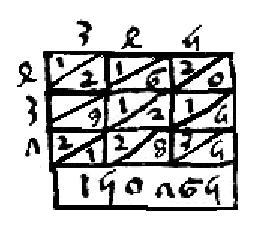
\includegraphics[width=5cm]{Nombres_et_calculs_did/Images/Num3_activites_Pamiers}}
\end{minipage}
\begin{minipage}{5cm}
\begin{pspicture}(-1,-1.5)(4,4)
   \psset{yunit=0.86,xunit=1.33}
   \multido{\n=0+1}{4}{\psline(\n,0)(\n,3)}
   \multido{\n=-1+1}{5}{\psline(0,\n)(3,\n)}
   \psline(1,3)(0,2)
   \psline(2,3)(0,1)
   \psline(3,3)(0,0)
   \psline(3,2)(1,0)
   \psline(3,1)(2,0) 
   \psline(0,-1)(0,0)
   \psline(3,-1)(3,0)
\end{pspicture}
\end{minipage}
\end{exercice*}

